\documentclass[sigconf,review,anonymous]{acmart}
% \documentclass[sigconf,nonacm]{acmart}


% Title portion
\title{Hermes: Bridging Relational and Algebraic Abstractions in Homomorphically Encrypted Databases}

\author{Dongfang Zhao}
\affiliation{
  \institution{Tacoma School of Engineering and Technology}
  \institution{Paul G. Allen School of Computer Science \& Engineering}
  \city{University of Washington}
  \country{United States}
}
\email{dzhao@cs.washington.edu}

\usepackage{multirow}

\usepackage[ruled,vlined,linesnumbered]{algorithm2e}
\usepackage{amsmath} % For advanced math commands
\newcommand{\don}[1]{\textcolor{magenta}{Dongfang: #1}}
\settopmatter{printfolios=true}

\usepackage{listings}
\usepackage{xcolor}

\lstdefinelanguage{SQL}{
  morekeywords={SELECT,FROM,WHERE,ORDER,BY,LIMIT,AND,OR,NOT,AS,ON,IN,IS,NULL,JOIN,LEFT,RIGHT,OUTER,INNER,GROUP,HAVING,ENC,Enc},
  sensitive=false,
  morecomment=[l]{--},
  morestring=[b]',
}

\lstset{
  language=SQL,
  basicstyle=\ttfamily\small,
  keywordstyle=\color{blue}\bfseries,
  commentstyle=\color{gray}\itshape,
  stringstyle=\color{teal},
  breaklines=true,
  columns=fullflexible,
  showstringspaces=false,
  frame=single,
  backgroundcolor=\color{gray!5},
  captionpos=b
}


\begin{document}

\begin{abstract}
Fully Homomorphic Encryption (FHE) promises the ability to compute over encrypted data without revealing sensitive contents. Yet, integrating it into real-world relational databases remains elusive due to prohibitive performance overhead and the structural mismatch between mutable database records and static ciphertexts. This paper presents Hermes, a system that enables homomorphically encrypted vectorized relational queries directly inside a standard SQL engine. To bridge the relational and algebraic abstractions, Hermes introduces a SIMD-aware data model that packs multiple records per ciphertext. By embedding precomputed aggregate statistics alongside data slots, the system supports efficient rotation-free aggregations. Furthermore, to overcome ciphertext immutability, we develop data-oblivious homomorphic algorithms based on slot masking and shifting, enabling secure in-place record modifications. Hermes is implemented as native loadable functions in MySQL, requiring no changes to the query planner or execution engine. Extensive evaluations on diverse datasets demonstrate up to 1600x higher throughput in encryption and over 30x speedup in insertion compared to conventional FHE implementations.
\end{abstract}

% \begin{teaserfigure}
%   \centering
%   \includegraphics[width=\linewidth]{dummy.png}
%   \caption{Hermes architecture overview.}
%   \label{fig:teaser}
% \end{teaserfigure}

\keywords{Database security, Fully homomorphic encryption, User-defined functions}

\begin{CCSXML}
<ccs2012>
  <concept>
    <concept_id>10.1145/1234</concept_id>
    <concept_desc>Security and privacy~Cryptography</concept_desc>
    <concept_significance>500</concept_significance>
  </concept>
  <concept>
    <concept_id>10.1145/5678</concept_id>
    <concept_desc>Information systems~Database management systems</concept_desc>
    <concept_significance>500</concept_significance>
  </concept>
</ccs2012>
</CCSXML>
\end{CCSXML}

\ccsdesc[500]{Security and privacy~Cryptography}
\ccsdesc[500]{Information systems~Database management systems}

\maketitle

\section{Introduction}

\subsection{Background and Motivation}

For over four decades, database systems have formed the backbone of modern data infrastructure, enabling structured storage, efficient retrieval, and scalable analytics. As the industry has transitioned to cloud-first architectures, the confidentiality of outsourced data has become a central concern. Increasingly, users demand end-to-end cryptographic protection throughout the entire computation pipeline, rather than merely during transmission or at rest.
Among cryptographic primitives, Fully Homomorphic Encryption (FHE) offers a mechanism to evaluate algebraic operations directly on encrypted data, removing the requirement to trust the compute server. Following Gentry's seminal construction~\cite{gentry2009}, subsequent schemes such as BFV and CKKS~\cite{FV2012,ckks2016} have improved computational efficiency and implementation maturity~\cite{openfhe}. FHE is now applied in practical domains, including secure machine learning and privacy-preserving analytics~\cite{boemer2020mp2ml,han2023}.

However, relational database systems have yet to fully integrate native homomorphic encryption. Although extensive research exists on encrypted databases~\cite{otawose_sigmod23,popa2011cryptdb,arx_vldb19}, current practical systems frequently leak access patterns through auxiliary indices or transfer the computational workload back to the client. Operating a relational engine directly on semantically secure ciphertexts remains an open challenge.
This limitation stems from a structural mismatch between database semantics and homomorphic computation. Traditional database management systems are designed for mutable records, evolving schemas, and runtime query execution plans. In contrast, FHE schemes operate over static circuits and immutable ciphertexts.
Resolving this structural divide requires more than wrapping FHE function calls within SQL. It necessitates a system architecture that maps the operational dynamics of relational execution to the algebraic invariants of encrypted computation. Without bridging these abstractions, applying cryptographic schemes to secure query processing remains impractical.

Given the availability of deployable FHE toolchains and the rising expectation for secure cloud analytics, the focus of system design is determining how relational databases can integrate homomorphic execution through a native interface. This work presents a principled step toward answering that question.

\subsection{Proposed Work}

We present \emph{Hermes}, a database subsystem that enables secure and efficient vectorized relational query execution over homomorphically encrypted data. Built atop the multi-slot capabilities of modern FHE schemes, Hermes is implemented as a suite of native MySQL loadable functions interfacing with OpenFHE~\cite{openfhe}. It addresses the structural mismatch between mutable relational records and static ciphertexts by contributing three core components:

\paragraph{(1) SIMD-aware Relational Data Model.}
Hermes adopts a packed ciphertext representation that maps multiple database tuples into parallel homomorphic slots. To accelerate homomorphic aggregation, the system reserves a specific slot within each ciphertext to store a precomputed auxiliary local sum over the data slots. This value is computed at packing time and maintained incrementally. By embedding this analytic state directly into the physical layout, encrypted aggregation queries such as \texttt{SUM} can be answered using constant-time ciphertext additions rather than expensive Galois rotations. This layout amortizes encryption overhead and improves both throughput and storage efficiency.

\paragraph{(2) Data-Oblivious Mutability Primitives.}
To overcome ciphertext immutability, Hermes supports dynamic record-level modifications directly on packed ciphertexts. Insertions and deletions are executed via homomorphic shift-and-mask operations. Inserting a new record shifts a tail segment rightward, while deleting a record shifts the segment leftward to clear the target slot. These structural updates are performed using homomorphic masking and slot-wise addition without requiring decryption or plaintext recovery. Such operations preserve semantic security and enable efficient in-place mutability while keeping the database access patterns completely opaque to the server.

\paragraph{(3) FHE-Native Query Engine Integration.}
Hermes facilitates a full-stack encrypted query execution pipeline without modifying the core MySQL engine or query planner. The system is realized as a collection of C++ modules compiled against OpenFHE and registered via the MySQL user-defined function interface. During ingestion, records are packed into ciphertexts with embedded auxiliary sums and stored as string-encoded blobs. At query time, the system executes relational operators entirely within the encrypted domain. This architecture avoids client-side orchestration and minimizes ciphertext transformations, delivering a performant and secure relational execution engine natively within the database management system.

In Summary, this paper makes the following contributions:

\begin{itemize}
    \item We formalize a vectorized ciphertext encoding that embeds precomputed aggregate statistics, reducing homomorphic aggregation from costly Galois rotations to constant-time additions and amortizing overall encryption overhead.

    \item We develop homomorphic shift-and-mask algorithms to achieve in-place slot-level insertions and deletions, enabling dynamic record mutability while preserving strict semantic security.

    \item We implement Hermes as a native MySQL extension to execute homomorphic query pipelines entirely within the DBMS. Extensive evaluations demonstrate up to 1,600x higher encryption throughput and 30x insertion speedup compared to conventional FHE implementations.
\end{itemize}

\section{Related Work and Preliminaries}

\subsection{Encrypted Databases}

One major class of encrypted databases relies on client-side processing, where query execution is deferred until the encrypted data is downloaded to a trusted local environment~\cite{akavia_sec23}. While this architecture strictly minimizes trust assumptions by keeping all analytical logic away from the cloud provider, it inherently sacrifices the computational benefits of server-side scalability. Transferring large volumes of encrypted records across the network incurs severe bandwidth penalties and high latency, effectively reducing the cloud database management system to a passive storage repository rather than an active execution engine.

An alternative approach attempts to split query execution between the client and the server, as seen in earlier information-hiding systems~\cite{hhaci_sigmod02}. In this model, server-side filters retrieve encrypted tuples guided by secure indices or cryptographic tokens generated by the client. Building upon this paradigm, systems like CryptDB~\cite{popa2011cryptdb}, Arx~\cite{arx_vldb19}, and Symmetria~\cite{symmetria_vldb20} explore different structural trade-offs between query functionality and data leakage. They employ layered encryption onions, partitioned data encodings, or specialized cryptographic circuits to evaluate relational predicates. However, these designs frequently leak access patterns or require multiple rounds of network interaction, as the server must often return intermediate candidate sets for the client to decrypt, refine, and re-upload.

More recently, homomorphic encryption has been integrated directly into encrypted database systems to compute over ciphertexts without continuous client intervention. For instance, Symmetria~\cite{symmetria_vldb20} utilizes multiplicative homomorphic encryption combined with additive extensions, whereas Rache~\cite{otawose_sigmod23} leverages layout-aware ciphertext placement alongside SIMD-optimized key switching techniques. Additional efforts from the applied cryptography community, such as HE3DB~\cite{10.1145/3576915.3616608} and ArcEDB~\cite{10.1145/3658644.3670384}, introduce new arithmetic and logic operators to accelerate SQL evaluations over ciphertexts. However, these solutions often manifest as standalone programmatic scripts rather than being fully integrated into a standard relational database engine. Furthermore, to mitigate the extreme performance penalties and noise growth of FHE, recent query engines like NSHEDB~\cite{jung2026nshedbnoisesensitivehomomorphicencrypted} rely on word-level leveled homomorphic encryption. Despite these cryptographic advances, existing homomorphic databases typically operate on scalar records, encrypting individual database attributes into isolated ciphertexts. This scalar approach fails to exploit the parallel processing capabilities of modern FHE schemes, leading to substantial storage inflation and computational bottlenecks during query execution. 

Hermes differs from prior systems by integrating homomorphic encryption directly into the ingestion path.
Unlike approaches that rely on client-side ciphertext generation or immutable payload storage, Hermes exposes SQL-level UDFs for packing, encrypting, and mutating ciphertexts at runtime.
Our system introduces a slot-aware data model that supports in-place ciphertext updates and maintains per-group local aggregates as part of the packing process.

\subsection{Fully Homomorphic Encryption}
\label{sec:prelim-he}

Homomorphic encryption (HE) enables computation on encrypted data without decryption. The seminal work by Gentry~\cite{gentry2009} introduced the first fully homomorphic encryption (FHE) scheme, laying the foundation for later constructions such as BFV~\cite{FV2012,brakerski2012}, GSW~\cite{gsw13}, BGV~\cite{BGV2014}, and CKKS~\cite{ckks2016}.  TFHE~\cite{torusCircuit} supports Boolean circuits and has seen recent improvements in bootstrapping performance~\cite{IEEETfhe,Guimares2024MOSFHETOS}. These schemes have been implemented in libraries including SEAL~\cite{sealcrypto}, HElib~\cite{helib}, OpenFHE~\cite{openfhe}, and LattiGo~\cite{lattigo_github}.


Hermes is built atop the BFV scheme~\cite{FV2012}, a lattice-based fully homomorphic encryption (FHE) construction supporting exact arithmetic over integers modulo a plaintext modulus \( t \). Let \( R = \mathbb{Z}[X]/(X^N + 1) \) be a cyclotomic ring of degree \( N = 2^k \) for some \( k \in \mathbb{N} \). A plaintext message is represented as an element of \( R_t := R / tR \), while ciphertexts reside in \( R_q^2 \), where \( q \gg t \) is a large ciphertext modulus.

A key feature of BFV is its support for \emph{plaintext packing} via the Chinese Remainder Theorem (CRT). When \( t \equiv 1 \mod 2N \), the ring \( R_t \) splits as a direct product of \( n = N/2 \) slots:
\[
R_t \cong \mathbb{Z}_t^n,
\]
enabling SIMD-style evaluation of vectorized inputs. Each plaintext \( \mathbf{m} = (m_0, \dots, m_{n-1}) \in \mathbb{Z}_t^n \) is encoded into a single polynomial \( m(X) \in R_t \), encrypted as \( \mathsf{Enc}(m) = \mathbf{c} \in R_q^2 \), and evaluated homomorphically across all slots.

Homomorphic operations preserve slot-wise semantics:
\begin{align*}
\mathsf{EvalAdd}(\mathsf{Enc}(\mathbf{m}), \mathsf{Enc}(\mathbf{m'})) &= \mathsf{Enc}(\mathbf{m} + \mathbf{m'}), \\
\mathsf{EvalMult}(\mathsf{Enc}(\mathbf{m}), \mathsf{Enc}(\mathbf{m'})) &= \mathsf{Enc}(\mathbf{m} \cdot \mathbf{m'}),
\end{align*}
where the arithmetic is component-wise modulo \( t \). In addition, the BFV scheme supports automorphism-based rotation operations, also known as \emph{Galois rotations}, which cyclically shift slot positions:
\[
\mathsf{EvalRotate}(\mathsf{Enc}(\mathbf{m}), r) = \mathsf{Enc}((m_{(i+r) \bmod n})_{i=0}^{n-1}).
\]

Hermes leverages this packing structure to encode multiple database tuples into a single ciphertext. This design enables parallel evaluation, slot-wise updates, and sublinear aggregation. Importantly, all packing and update logic remains entirely within the encrypted domain, without leaking intermediate values or structural metadata.

In addition, the BFV scheme supports automorphism-based slot rotation using Galois group actions. For any \( r \in \mathbb{Z} \), a cyclic slot rotation is realized via the Galois automorphism \( \sigma_r: X \mapsto X^r \mod (X^N + 1) \), which acts on ciphertexts by permuting their internal slot layout. To evaluate this transformation homomorphically, the client must precompute and upload the corresponding Galois keys:
\[
\mathsf{EvalAtIndex}(\mathsf{Enc}(\mathbf{m}), r) = \mathsf{Enc}((m_{(i+r)\bmod n})_{i=0}^{n-1}),
\]
where the rotation index \( r \) corresponds to a specific automorphism in the Galois group \( \operatorname{Gal}(R_q / \mathbb{Q}) \). These keys enable Hermes to perform selective slot access, masking, and reorganization within encrypted vectors while preserving semantic security.

% \subsection{Provable Security}
% \label{sec:prelim-security}

% Semantic security for public-key encryption is captured by the notion of indistinguishability under chosen-plaintext attack (IND-CPA). Let $\Pi = (\mathsf{KeyGen},\ \mathsf{Encrypt},\ \mathsf{Decrypt},\ \mathsf{EvalAdd},\ \mathsf{EvalMult})$ be a probabilistic encryption scheme defined over a message space $\mathcal{M}$ and a ciphertext space $\mathcal{C}$. The scheme $\Pi$ is IND-CPA secure if no probabilistic polynomial-time (PPT) adversary can, with non-negligible advantage, distinguish between the encryptions of any two chosen messages in $\mathcal{M}$.

% Formally, consider the following security game between a challenger \( \mathcal{C} \) and an adversary \( \mathcal{A} \):

% \begin{enumerate}
%   \item The challenger generates a key pair \( (\mathsf{pk}, \mathsf{sk}) \leftarrow \mathsf{KeyGen}(\lambda) \) for security parameter \( \lambda \), and sends \( \mathsf{pk} \) to \( \mathcal{A} \).
%   \item The adversary chooses two equal-length messages \( m_0, m_1 \in \mathcal{M} \) and submits them to \( \mathcal{C} \).
%   \item The challenger samples a uniform bit \( b \in \{0,1\} \), computes \( c^* \leftarrow \mathsf{Encrypt}_{\mathsf{pk}}(m_b) \), and returns \( c^* \) to \( \mathcal{A} \).
%   \item The adversary outputs a guess \( b' \in \{0,1\} \).
% \end{enumerate}

% The scheme is IND-CPA secure if, for all PPT adversaries \( \mathcal{A} \),
% \[
% \left| \Pr\left[ \mathcal{A}(\mathsf{pk}, c^*) = b \right] - \frac{1}{2} \right| < \varepsilon(\lambda),
% \]
% where \( \varepsilon \) is a negligible function in \( \lambda \).

% Modern fully homomorphic encryption schemes such as BFV, BGV, and CKKS satisfy IND-CPA under the hardness assumption of the Ring Learning With Errors (RLWE) problem. For these schemes, the encryption process is randomized: each plaintext message is masked with independently sampled noise and embedded in a structured polynomial ring, ensuring ciphertext distributions are computationally indistinguishable from random.

% The multi-slot encoding structure introduced in BFV and related schemes does not weaken IND-CPA security. A vector \( \mathbf{m} = (m_0, \dots, m_{n-1}) \in \mathcal{M}^n \) is encrypted into a single ciphertext \( c \in \mathcal{C} \), but as long as \( \mathsf{Encrypt} \) remains probabilistic and the adversary lacks access to decryption oracles, semantic security extends to the full plaintext vector.

% Subsequent homomorphic operations (e.g., addition, multiplication, rotation) are performed over ciphertexts without leaking intermediate plaintexts. Since the adversary cannot observe any result of decryption or affect the noise distribution, the composed evaluation remains semantically secure under standard composition theorems.

% This security model provides the foundation upon which encrypted database systems can be constructed: so long as no decryption is performed server-side, and all query logic is implemented using semantically secure operations, the confidentiality of underlying plaintexts is preserved.

% \subsection{MySQL User-Defined Functions (UDFs)}
% \label{sec:prelim-udf}

% MySQL supports native extensibility through \emph{User-Defined Functions} (UDFs), which allow developers to register custom functions written in C/C++ as shared objects. Once registered, a UDF can be invoked in SQL queries as a first-class function, operating over tuples during query execution.

% A typical scalar UDF consists of the following exported routines:
% \begin{itemize}
%   \item \texttt{foo\_init} \quad ($\mathtt{foo\_init}$): initializes internal memory and checks argument types.
%   \item \texttt{foo} \quad ($\mathtt{foo}$): performs the main per-tuple computation.
%   \item \texttt{foo\_deinit} \quad ($\mathtt{foo\_deinit}$): releases allocated memory and closes resources.
% \end{itemize}

% Aggregate UDFs additionally implement:
% \begin{itemize}
%   \item \texttt{foo\_add} \quad ($\mathtt{foo\_add}$): accumulates intermediate results across tuples.
%   \item \texttt{foo\_clear}, \texttt{foo\_reset} \quad ($\mathtt{foo\_clear}, \mathtt{foo\_reset}$): manage state lifecycle during grouping.
% \end{itemize}

% Each UDF receives input arguments via the \texttt{UDF\_ARGS} structure, which exposes parameter values and types through typed pointers. Output is returned through a caller-allocated buffer and must specify an explicit output length. All memory is managed manually, and no standard C++ types (e.g., \texttt{std::string}) may be used within the interface boundary.

% This plugin model maps naturally to encrypted computation. The per-tuple stateless execution model aligns with ciphertext-level operations, while aggregate UDF hooks enable accumulation over encrypted records. Importantly, UDFs operate entirely inside the database engine, avoiding the need for external processes or client-managed cryptographic operations.

% Hermes implements each homomorphic operation as a standalone UDF module, ensuring modularity and compatibility with SQL queries. Operations such as encryption, slot-wise insertion, and encrypted summation are exposed as standard SQL functions, compiled into dynamically loadable \texttt{.so} libraries. This design permits seamless integration with the MySQL query planner and execution engine, bridging encrypted computation with traditional relational workflows.

\subsection{Alternative Secure Processing Paradigms}

Alongside purely cryptographic storage, trusted hardware enclaves provide an alternative route for secure data processing. Systems utilizing Intel SGX such as ObliDB~\cite{10.14778/3364324.3364331} and CryptSQLite~\cite{8946540} protect data in memory while offering oblivious query processing to prevent access pattern leaks. Enterprise solutions have also adopted this paradigm. For instance, recent iterations of Azure SQL Database~\cite{10.1145/3318464.3386141} leverage enclaves to enable rich pattern matching over encrypted columns. Furthermore, hardware isolation techniques have been proposed to secure peripheral interfaces and web environments against side channel attacks~\cite{8835331}. While enclaves deliver high performance, they introduce strict hardware dependencies and remain vulnerable to sophisticated microarchitectural exploits, which pure homomorphic encryption avoids.

Another prominent paradigm involves Secure Multi-party Computation and federated privacy. Frameworks like Conclave~\cite{10.1145/3302424.3303982} and Shrinkwrap~\cite{10.14778/3291264.3291274} accelerate analytics over big data by partitioning queries between cleartext local processing and secure protocols. Similarly, advanced join aggregate queries can be evaluated across private datasets without exposing individual records~\cite{10.1145/3448016.3452808}. Managing cross cryptographic leakages in such distributed databases is a complex endeavor~\cite{10598104}. Additionally, massive parallel query optimization strategies~\cite{10.1145/2038916.2038928} and Private Information Retrieval~\cite{10.1109/TKDE.2012.90} remain essential for scalable data extraction. However, multi-party protocols inherently require heavy network synchronization among non-colluding servers, which is a fairly strong assumption that may or may not hold for many practical scenarios. Hermes bypasses these communication bottlenecks by shifting the computational burden entirely to the server side evaluation of SIMD packed ciphertexts.

\subsection{Terminology and Notation}
\label{sec:prelim-notation}

We summarize key terms and notation used throughout this paper. Let $n$ denote the number of slots supported by the plaintext modulus and ring parameters of the BFV encryption scheme. All vectors are implicitly assumed to be over $\mathbb{Z}_t^n$, where $t$ is the plaintext modulus.

\begin{itemize}
  \item \textbf{Slot:} Each ciphertext encodes a vector of $n$ plaintext elements, known as \emph{slots}. Slots are independently addressable under SIMD operations supported by BFV.

  % \item \textbf{Ciphertext:} A ciphertext $c \in \mathcal{C}$ is a BFV-encoded object that homomorphically encrypts $[m_0, \dots, m_{n-1}]$ for some plaintext values $m_i \in \mathbb{Z}_t$. Ciphertexts may undergo operations such as addition, multiplication, and automorphic permutation.

  \item \textbf{Group ID:} In Hermes, input tuples are partitioned by a logical \emph{group ID}, which assigns each record to a packed vector instance. All records within the same group are encoded into the same ciphertext. The mapping from record to group is deterministic and index-driven.

  \item \textbf{Auxiliary Sum Slot:} Hermes reserves the final slot (slot $n{-}1$) in each ciphertext to store the \emph{local sum}, i.e., the plaintext sum $\sum_{j=0}^{n-2} m_j$ of all payload slots. This value is computed at packing time and used to accelerate encrypted aggregation without Galois rotation.

  \item \textbf{Packed Representation:} A ciphertext that stores $n{-}1$ application values and one auxiliary statistic is referred to as a \emph{packed representation}. This format enables efficient updates and aggregation via SIMD-aware primitives.

  \item \textbf{Logical Length:} Some plaintext vectors do not occupy all $n$ slots. The number of meaningful entries is called the \emph{logical length}, and is used to control serialization, summation, and slot masking operations.
\end{itemize}

\section{Hermes: FHE Layer for Vectorized Tuples}

Hermes is designed as a MySQL-integrated system with a new data abstraction for storing, updating, and querying encrypted relational data via fully homomorphic encryption (FHE). It is built upon the multi-slot property of lattice-based FHE schemes (e.g., BFV), where a single ciphertext can encode a vector of plaintexts. This allows Hermes to pack multiple database records into a single ciphertext, enabling efficient SIMD-style operations. To support dynamic updates, we develop homomorphic algorithms for inserting and deleting records within packed ciphertexts without decryption. Additionally, we maintain auxiliary local sums within the ciphertext layout to accelerate aggregate queries. The following sections detail the design of Hermes's packed ciphertext data model and the homomorphic primitives for mutability. 

\subsection{Packed Ciphertext Data Model}

We propose a new packing-based layout where each ciphertext holds a fixed-size group of database records. This model amortizes encryption cost and supports efficient SIMD-style processing. To enable insert and delete operations over individual slots, we design a homomorphic slot manipulation interface that combines masking, shifting, and slot-zeroing operations, all within the ciphertext algebra. Unlike conventional systems that require decryption and re-encryption for each update, our design ensures that updates can be applied entirely in the encrypted domain.

\subsubsection{Slot-Aware Packing Strategy}

In Hermes, we introduce a structured packing layout that enables efficient storage and manipulation of encrypted data within the SIMD-style slot architecture of the BFV homomorphic encryption scheme. Rather than encrypting each tuple into a separate ciphertext, which incurs significant memory and performance overhead, we adopt a batched layout where each ciphertext encodes a fixed-size vector of plaintext values, referred to as \emph{slots}.

Let $N$ denote the ring dimension of the BFV scheme. When batching is enabled (via the Chinese Remainder Theorem on cyclotomic rings), the scheme yields $n = N/2$ usable slots. For example, with $N=8192$, Hermes can store $n = 4096$ individual scalar values per ciphertext. However, instead of utilizing all $n$ slots for raw data, we reserve one designated slot (typically the last) to store an auxiliary value, such as the \emph{local sum} of the vector entries. This yields an effective capacity of $n-1$ logical records per ciphertext.

Each slot in a packed ciphertext has a fixed positional meaning: slot $i$ corresponds to the $i$-th logical record in the group. This deterministic alignment enables precise slot-wise reasoning and efficient update semantics. When a ciphertext is decrypted, the unpacked vector reveals values at well-defined offsets, allowing Hermes to reconstruct the plaintext table fragment without additional metadata. This position-indexed design is critical for supporting secure in-place modifications, such as insertions and deletions, without leaking tuple identity or requiring explicit key-column mapping.

Formally, a packed ciphertext $c$ in Hermes can be viewed as a vector:
\[
c = \text{Enc}([v_0, v_1, \dots, v_{n-2}, \sigma]),
\]
where $v_i$ is the plaintext value in logical slot $i$, and $\sigma$ is the slot reserved for auxiliary information, such as $\sigma = \sum_{i=0}^{n-2} v_i$ in the case of sum queries.

Compared to traditional row-wise encryption, this layout significantly improves storage density and amortizes encryption cost across multiple tuples. It also enables efficient homomorphic operations such as component-wise masking, conditional updates, and encrypted aggregation over slots. In essence, we reinterpret ciphertexts as \emph{relational vectors} whose entries correspond to logical rows in a database group, thereby enabling vectorized query execution over encrypted domains.

\subsubsection{Homomorphic Insertion}

Hermes supports in-place insertion of plaintext values into packed ciphertexts without requiring decryption or client-side re-encryption. The goal is to insert a new value $v$ into logical slot $i$ of an existing ciphertext $c$, where slots $i$ through $n-2$ may already contain data. Since ciphertexts are encoded as vectors of fixed size, insertion requires shifting all subsequent entries rightward by one position to make room for the new value. This is analogous to an in-place insert into an array but performed entirely under encryption.

The insertion procedure consists of three homomorphic operations: (1) Galois rotation, (2) plaintext masking, and (3) ciphertext addition. We first perform a Galois right-rotation on $c$, yielding a new ciphertext $c_{\text{rot}}$ in which all slots are shifted by one position. However, this operation naively shifts all slots, including the local sum at slot $n-1$, which must be preserved. Therefore, Hermes applies a plaintext mask $m_{\text{preserve}}$ to $c$ before rotation to ensure that only slots $i$ through $n-2$ are moved. This yields a masked-and-rotated ciphertext $c_{\text{shifted}}$ in which slot $i$ is now vacant.

Next, the new plaintext value $v$ is embedded into a one-hot plaintext vector $m_v$ where $m_v[i] = v$ and $m_v[j] = 0$ for $j \ne i$. This mask is encrypted into $c_v$, a ciphertext containing $v$ only at the desired slot. Finally, we compute:
\[
c' = \text{EvalAdd}(c_{\text{shifted}}, \text{EvalMult}(c_v, m_i)),
\]
where $m_i$ is a binary plaintext mask that ensures $v$ is added only at slot $i$. This avoids interference with other slots.

In addition to updating the main data slots, Hermes updates the local sum $\sigma$ stored at slot $n-1$. This is achieved via scalar plaintext addition:
\[
\sigma' = \text{EvalAddPlain}(\sigma, v).
\]
Since $v$ is known in plaintext, the update to the auxiliary slot incurs negligible overhead and does not require re-encryption.

It should be noted that this procedure is performed within the database server process using OpenFHE's C++ API, without leaking which slot was modified or what value was inserted. The result is a new ciphertext that logically contains all previous values, $v$ inserted at slot $i$, and an updated sum at slot $n-1$. This mechanism allows Hermes to support encrypted ingestion of streaming data with minimal cryptographic cost.

When a ciphertext pack reaches the maximum number of supported slots, no further insertions can occur without creating a new ciphertext. In Hermes, we adopt a conservative policy: each group is associated with a single ciphertext, and insertion beyond capacity is rejected. Future extensions may support \emph{chained packing}, where overflow records spill into a second ciphertext. However, doing so requires maintaining slot alignment metadata and reintroduces some of the per-ciphertext management overhead that Hermes aims to avoid.

\subsubsection{Homomorphic Deletion}

Hermes enables encrypted deletion over packed ciphertexts by simulating a logical left-shift over the underlying slots while preserving the ciphertext algebra. The goal is to remove the value at slot $i$ of ciphertext $c$, and to maintain a compacted layout where all subsequent values are shifted leftward and the last slot is cleared. Importantly, this is done entirely within the encrypted domain, without re-encoding the ciphertext or exposing the deletion position to the server.

The deletion procedure consists of three conceptual steps: (1) rotation, (2) masking, and (3) auxiliary slot update. First, Hermes isolates the subvector of ciphertext $c$ corresponding to slots $i+1$ through $n-2$ and rotates it leftward by one position. This is accomplished via a Galois left rotation:
\[
c_{\text{rot}} = \text{EvalRotate}(c, -1),
\]
followed by a masking step to ensure that only the intended region is affected. Specifically, a plaintext mask $m_{\text{shift}}$ is applied before rotation to preserve slot integrity and avoid accidental overwriting of unaffected entries.

Next, Hermes applies a zeroing mask $z$ to clear the final slot (slot $n-2$), which now contains a duplicate or stale value as a result of the shift. The mask $z$ is a binary plaintext vector where $z[j] = 1$ for $j < n-2$ and $z[n-2] = 0$, ensuring:
\[
c' = \text{EvalMult}(c_{\text{rot}}, z).
\]
The slot at index $i$, which originally contained the value to delete, has now been overwritten by the shifted entry from $i+1$, and the final slot is set to zero, restoring the invariant that only $n-1$ data entries are active.

Finally, the local sum maintained in slot $n-1$ is updated by subtracting the deleted plaintext value $v$. Since $v$ is assumed to be known at deletion time (e.g., from a query input), this update is executed via plaintext subtraction:
\[
\sigma' = \text{EvalSubPlain}(\sigma, v).
\]

All steps, including rotation, masking, and sum adjustment, are performed homomorphically within the database server using OpenFHE APIs. This design avoids decryption-reencryption cycles, ensures slot occupancy consistency, and maintains statistical privacy regarding which slot was deleted. As with insertion, the deletion logic treats ciphertexts as logical arrays and preserves relational semantics under homomorphic constraints.

When all payload slots in a packed ciphertext have been deleted, the ciphertext becomes logically empty, although its auxiliary sum slot may still contain residual values. In Hermes, such ciphertexts are treated as semantically inert: they contribute nothing to aggregate queries, and further deletions are treated as no-ops. However, the ciphertext itself is retained in the database to preserve structural consistency unless explicitly garbage-collected.
To maintain correctness, Hermes ensures that the auxiliary sum is updated to zero whenever the payload becomes empty. This guarantees that global aggregation remains accurate even in the presence of entirely deleted groups.

\subsection{Maintenance for Aggregate Queries}

To support efficient encrypted aggregation, Hermes maintains a running \emph{local sum} for each packed ciphertext. This design allows queries such as \texttt{SELECT SUM(attr)} or \texttt{GROUP BY key} to be evaluated via lightweight ciphertext addition without slot-wise traversal or Galois rotations. The remainder of this subsection describes how the local sum is constructed, maintained, and queried.

\subsubsection{Encoding at Packing Time}

Hermes adopts a hybrid encoding strategy in which each packed ciphertext stores not only a fixed-length array of plaintext values but also a precomputed auxiliary statistic: the sum of those values. This local sum is embedded into the last slot of the ciphertext at the time of packing, enabling efficient aggregation queries without the need for slot-wise traversal or ciphertext rotations (i.e., Galois automorphisms).

Given a batch of $n-1$ plaintext values $(v_0, v_1, \dots, v_{n-2})$ to be packed into a ciphertext, Hermes computes their sum $s = \sum_{i=0}^{n-2} v_i$ in plaintext and constructs an extended vector of the form:
\[
\mathbf{m} = (v_0, v_1, \dots, v_{n-2}, s) \in \mathbb{Z}_t^n,
\]
where $t$ is the plaintext modulus and $n$ is the total number of BFV batching slots (typically $n = N/2$ for a ring dimension $N$). The extended vector $\mathbf{m}$ is then passed to the OpenFHE API to generate a packed plaintext object Packed($\mathbf{m}$), which is encrypted into a ciphertext $c = \text{Encrypt}(pk, \text{Packed}(\mathbf{m}))$.

This packing layout effectively reserves the final slot (slot $n-1$) as a local accumulator, denoted as $\text{sum}_{\text{local}}$. Because BFV ciphertexts support SIMD-style processing, all data and the auxiliary sum coexist in a single ciphertext. Since the sum is computed before encryption, it incurs no additional homomorphic cost.

The benefit of this encoding is twofold. First, it amortizes the cost of sum computation over all packed values, reducing the number of ciphertexts needed for downstream aggregation. Second, it enables highly optimized aggregate queries, such as \texttt{SELECT SUM(attr)}, by reducing global summation to a single ciphertext-level addition over the final slot of each ciphertext. Instead of rotating and adding up all slots, the query planner only needs to sum the values at slot $n-1$ across all ciphertexts:
\[
\text{SUM(attr)} = \text{EvalAdd}(c_1[n{-}1], c_2[n{-}1], \dots, c_k[n{-}1]).
\]

This approach dramatically reduces computational complexity and latency, particularly when processing large encrypted datasets. By pre-allocating and embedding local statistics into the ciphertext layout, Hermes transforms aggregation from a slot-wise operation into a slot-agnostic one, leveraging the structure of FHE schemes for practical query acceleration.

\subsubsection{Aggregation Update}

While Hermes encodes a local sum at packing time, database workloads often require dynamic updates. To ensure the correctness of aggregation queries over mutable encrypted data, we design a lightweight incremental strategy to maintain the local sum as records are inserted or deleted. This strategy preserves consistency between the payload slots and the auxiliary sum slot, while avoiding costly recomputation or re-encryption.

Consider a ciphertext $c$ whose first $n-1$ slots contain encrypted values $(v_0, \dots, v_{n-2})$, and whose final slot (slot $n-1$) stores the corresponding local sum $s = \sum_{i=0}^{n-2} v_i$. When a new value $v_{\text{new}}$ is inserted into the payload (e.g., at slot $i$), Hermes also adds $v_{\text{new}}$ into the local sum via scalar plaintext addition. This is performed by constructing a plaintext vector $\mathbf{m}_{\text{aux}}$ such that:
\[
\mathbf{m}_{\text{aux}} = (0, 0, \dots, 0, v_{\text{new}}),
\]
where only the final slot is nonzero. Then the updated ciphertext $c'$ is computed homomorphically as:
\[
c' = \text{EvalAdd}(c, \mathbf{m}_{\text{aux}}).
\]
This operation increases the local sum while preserving the rest of the payload unchanged. Note that no re-encryption is required, and the update remains entirely within the ciphertext space.

A similar process applies to deletions. Suppose a value $v_{\text{del}}$ is removed from a known slot. Hermes constructs a plaintext subtraction mask $\mathbf{m}_{\text{aux}}'$ where:
\[
\mathbf{m}_{\text{aux}}' = (0, 0, \dots, 0, -v_{\text{del}}),
\]
and applies:
\[
c' = \text{EvalAdd}(c, \mathbf{m}_{\text{aux}}').
\]
The net effect is that the auxiliary slot now holds the correct sum of the modified payload. Since inserted and deleted values are supplied in cleartext as part of the query expression, this approach avoids the overhead of decrypting and summing the full ciphertext.

This fine-grained sum adjustment strategy is a key enabler of real-time encrypted aggregation. It ensures that the auxiliary slot always remains synchronized with the payload, supporting fast `GROUP BY' and `SUM' queries without compromising correctness or requiring client interaction. All updates are executed inside SQL statements via homomorphic functions (e.g., MySQL UDFs) and do not reveal which slot was updated.

\subsection{Security and Correctness Analysis}

We provide a formal security analysis of Hermes under the standard IND-CPA model. Our design avoids client-server interaction after encryption and ensures that all slot-level operations are data-independent, thereby preventing leakage from slot position, access pattern, or update frequency. We further prove that the packed representation with embedded statistics does not weaken the semantic security of the base FHE scheme, and our masking/shift update primitives are indistinguishable under standard lattice assumptions.

\subsubsection{Security Model and Assumptions}

We analyze the security of Hermes under the standard indistinguishability under chosen-plaintext attack (IND-CPA) model, instantiated using BFV~\cite{FV2012}. We assume a passive, honest-but-curious adversary with full access to encrypted database contents, including ciphertexts before and after updates, as well as query results. The adversary may observe ciphertext structure, slot layout, and numerical patterns in decrypted outputs but is assumed to follow protocol without actively deviating from the query logic. However, the server does not record low-level timing, memory access, or power traces: Preventing side-channel attacks is beyond the scope of this work.

In order to ensure that Hermes does not introduce any new leakage channels beyond what is inherent in the underlying FHE scheme, we require the following invariants to hold:

\begin{enumerate}
  \item \textit{Indistinguishability of Ciphertexts:} For any two payload vectors $v$ and $v'$ of the same length, their packed ciphertexts $c = \texttt{Encrypt}(v)$ and $c' = \texttt{Encrypt}(v')$ are computationally indistinguishable under the IND-CPA security of BFV.
  
  \item \textit{Update Pattern Privacy:} Insertion and deletion operations do not reveal the affected slot position or the identity of the modified value to the server. That is, for any two slots $i$ and $j$, the adversary cannot distinguish an insertion at slot $i$ from one at $j$ by examining ciphertext differences alone.

  \item \textit{Aggregation Consistency:} Global aggregation over auxiliary slots (e.g., encrypted `SUM') reveals no more information than the final aggregate result; the per-ciphertext local sum values are protected under the encryption scheme.

  \item \textit{No Adaptive Leakage:} Hermes does not reveal any intermediate plaintexts or randomness that could be used to link ciphertexts over time. All operations are performed homomorphically and reuse no client secrets post-encryption.
\end{enumerate}

Importantly, the Hermes data model and update interface preserve these properties without relying on secure multi-party computation (MPC), secure enclaves, or trusted client-side computation. All operations, such as packing, insert/delete, and aggregation, are fully executed on encrypted data within the untrusted database server.

This model captures realistic cloud deployment scenarios where users outsource encrypted databases to an untrusted cloud provider but wish to retain strong confidentiality guarantees under standard cryptographic assumptions (e.g., Ring-LWE hardness). We note that this threat model is stronger than many property-preserving encryption (PPE) systems, which often leak order, frequency, or access pattern by design.

\subsubsection{Preservation of IND-CPA Security}

The semantic security of Hermes relies on the assumption that the underlying BFV scheme remains IND-CPA secure under all ciphertext manipulations performed in the system. This includes ciphertext packing, masked updates, homomorphic insertion and deletion, and the embedding of auxiliary local statistics such as the group sum. We now argue that Hermes does not introduce any structural leakage or functional dependencies that could be exploited to distinguish ciphertexts. The formal proof is based on the following two observations.

First, although Hermes embeds deterministic metadata (e.g., local sums) into specific slots, the entire ciphertext is encrypted using randomized BFV encryption over the full plaintext vector. IND-CPA security guarantees that the ciphertext remains indistinguishable even if some slots are derived from others, so long as the message vector is encrypted as a whole with fresh randomness. In particular, the inclusion of auxiliary statistics does not compromise the semantic security of any individual slot.

Second, Hermes performs all slot-level updates, such as insertion and deletion, purely through homomorphic operations. These updates use masking, shifting, and slot-wise additions, but never invoke decryption, re-encryption, or key switching. No new randomness is injected, and no plaintext values are revealed or reconstructed during runtime. As a result, each modified ciphertext maintains the same IND-CPA security level as its original version, with no additional leakage beyond the allowed ciphertext interface.

We start by recalling the notion of IND-CPA security.
\begin{definition}[IND-CPA Security]
Let $\mathsf{Enc}_\mathsf{pk}(m; r)$ denote the encryption of a plaintext $m$ under public key $\mathsf{pk}$ and randomness $r$. A scheme is IND-CPA secure if no probabilistic polynomial-time (PPT) adversary $\mathcal{A}$ can distinguish between encryptions of $m_0$ and $m_1$ for any chosen pair of equal-length plaintexts, even given arbitrary access to the encryption oracle. Formally, for any PPT adversary $\mathcal{A}$, the advantage
\[
\text{Adv}_\mathcal{A}^{\text{IND-CPA}} = \left| \Pr[\mathcal{A}(\mathsf{Enc}(m_0)) = 1] - \Pr[\mathcal{A}(\mathsf{Enc}(m_1)) = 1] \right|
\]
is negligible in the security parameter $\lambda$.
\end{definition}

\begin{lemma}
Let $\mathcal{C}$ be the set of ciphertexts generated and manipulated by Hermes. Then under the assumption that the base FHE scheme (BFV) is IND-CPA secure, the ciphertext $c \in \mathcal{C}$ remains IND-CPA secure throughout all operations in Hermes.
\end{lemma}

\begin{proof}
See Appendix.
\end{proof}

An important subtlety in Hermes is the deterministic embedding of auxiliary data into a fixed slot. While this creates a structural invariant, it does not violate IND-CPA since the data being embedded is functionally independent on other encrypted slots. From a cryptographic perspective, this corresponds to publishing a function $f(v_0, \dots, v_{n-2}) = s$ along with the encryption of the vector, which is a standard practice in FHE-based secure computation.
Furthermore, all masking and slot operations are purely homomorphic and do not involve conditional branching or secret-dependent control flow. No part of the computation leaks information via side channels, timing, or slot access patterns. 

\subsubsection{Update Privacy via Slot-Level Obfuscation}

To preserve data obliviousness within packed ciphertexts, Hermes ensures that individual insertions and deletions are indistinguishable with respect to their slot index. Since encrypted updates are performed via uniform homomorphic operations, namely Galois rotations, plaintext masking, and slot-wise additions, the adversary cannot determine which slot was modified given a before-and-after pair of ciphertexts. We formalize this guarantee using a slot-level indistinguishability game.

We start by formally defining the game.
\begin{definition}[Slot Update Indistinguishability Game]
Let $c$ be an encrypted packed ciphertext over $n$ slots under BFV. Consider two update positions $i_0, i_1 \in \{0, \dots, n-2\}$. The goal of the adversary $\mathcal{A}$ is to distinguish whether an insertion was applied at position $i_0$ or $i_1$. The game proceeds as follows:
\begin{enumerate}
  \item Challenger generates keypair $(\mathsf{pk}, \mathsf{sk}) \leftarrow \mathsf{KeyGen}(1^\lambda)$.
  \item Adversary chooses a plaintext vector $\vec{v} = (v_0, \dots, v_{n-2})$ and computes $c \leftarrow \mathsf{Enc}_\mathsf{pk}(\vec{v})$.
  \item Challenger chooses a random bit $b \in \{0,1\}$.
  \item Challenger inserts a known value $\delta$ at slot $i_b$ using Hermes' homomorphic insert logic, resulting in $c' = \mathsf{Insert}(c, i_b, \delta)$.
  \item Adversary is given $c'$ and outputs a guess $b' \in \{0,1\}$.
\end{enumerate}

We define the adversary's advantage as:
\[
\text{Adv}^{\text{slot-ins}}_\mathcal{A} = \left| \Pr[b' = b] - \frac{1}{2} \right|.
\]
Hermes guarantees slot-level update privacy if $\text{Adv}^{\text{slot-ins}}_\mathcal{A}$ is negligible in the security parameter $\lambda$.
\end{definition}

\begin{theorem}
If the underlying BFV encryption scheme is IND-CPA secure, then Hermes satisfies slot-update indistinguishability for any polynomial-time adversary $\mathcal{A}$.
\end{theorem}

\begin{proof}
See Appendix.
\end{proof}

It is important to note that Hermes maintains \textit{position-hiding homomorphism} not by permuting slot values, but by maintaining the slot structure while masking all auxiliary effects of an update. The Galois shift operator is position-invariant modulo a known offset; the zeroing mask ensures no unintentional data leaks from adjacent slots. The reserved auxiliary slot (e.g., local sum) is updated using scalar plaintext operations, and its growth reflects only the net value change, not the specific position of insertion or deletion. This makes Hermes suitable for applications requiring structural privacy in addition to semantic security.

\subsubsection{Correctness of Encrypted Updates and Aggregates}

We now formally prove that Hermes \emph{correctly} maintains the semantics of encrypted vector updates and aggregate computations in the presence of insertions and deletions. 

\begin{theorem}
  Hermes guarantees the following three properties for any sequence of homomorphic insertions, deletions, and global aggregations over packed ciphertexts:
  \begin{enumerate}
    \item The logical payload vector within each ciphertext remains consistent with the intended insertions and deletions, preserving the correct order and values of active slots.
    \item The auxiliary sum slot accurately reflects the current sum of all valid payload slots after any sequence of updates, ensuring that local statistics remain correct.
    \item The result of encrypted aggregation (e.g., $`SUM'$) over multiple ciphertexts yields the correct aggregate value corresponding to the underlying plaintexts, even in the presence of concurrent updates.
  \end{enumerate}
\end{theorem}

\begin{proof}
See Appendix.
\end{proof}

\section{System Implementation}

We implement \textsc{Hermes} as a suite of MySQL loadable functions written in C++ with OpenFHE v1.2.4. The system consists of modular components for slot-wise packing, homomorphic insertion and deletion, local-sum-aware aggregation, and slot-selective decryption, all of which are executed natively within the MySQL runtime.

As of March 2026, the codebase comprises 4761 lines of code. All components are implemented in C++ and compiled into dynamic libraries registered as MySQL UDFs. Our minimalist integration strategy avoids any modification to the MySQL source code or query engine internals. The full source code is publicly available on Github.
% \[
% \texttt{\url{https://github.com/hpdic/hermes}}
% \]
Experiments and development were partially supported by the NSF-funded Chameleon Cloud infrastructure~\cite{chameleoncloud}.

\subsection{Architecture and Integration}

Hermes is implemented as a runtime plugin using the MySQL User Defined Function (UDF) interface. Each cryptographic operation is compiled as a C++ function into a shared object \texttt{.so} file, which is dynamically linked into the MySQL server process at runtime. This mechanism preserves full compatibility with unmodified MySQL 8.x deployments, requiring no server side modifications or query proxies.

Each plugin function adheres strictly to the MySQL UDF lifecycle. The \texttt{\_init} function validates argument counts and types while allocating necessary internal states. The core execution resides in \texttt{\_func}, which runs per row during query evaluation. Finally, the optional \texttt{\_deinit} function releases allocated memory and handles. Hermes relies on this C interface to expose its cryptographic primitives to the SQL engine.

To bridge MySQL data types and OpenFHE plaintexts, all inputs undergo explicit parsing across the foreign function interface (FFI) boundary. MySQL UDF arguments arrive as raw C pointers tagged with type enumerations, such as \texttt{INT\_RESULT} or \texttt{STRING\_RESULT}. Hermes implements strict casting logic to convert these inputs into 64 bit signed integers, utilizing \texttt{std::istringstream} when numerical data is passed as string types. These scalar values are subsequently passed to the OpenFHE \texttt{MakePackedPlaintext} API.

Instead of serializing ciphertexts into strings or blobs for every operation, ciphertext objects are allocated on the heap and remain within the memory space of the MySQL process. For diagnostic and linkage purposes, Hermes returns a string encoded metadata footprint of the ciphertext rather than the serialized payload. This diagnostic string takes the format of \texttt{0xADDR (v, size=s)}, where \texttt{ADDR} is the hexadecimal memory address of the ciphertext object, \( v \in \mathbb{Z} \) is a verified decrypted payload used for internal sanity checks, and \( s \) represents the object footprint in bytes. This memory centric layout minimizes I/O overhead during query execution.

Integrating OpenFHE v1.2.4 requires specific dynamic linker configurations. Hermes statically compiles the necessary cryptographic modules and bundles them into a relocatable shared object. At runtime, dependencies like \texttt{libOPENFHEcore.so} are copied into the MySQL plugin directory. To make these visible to the \texttt{mysqld} daemon, an injected \texttt{LD\_LIBRARY\_PATH} is configured via a \texttt{systemd} override file. This deployment strategy ensures correct dynamic linking on Ubuntu 24.04 LTS environments and prevents unresolved symbol errors during plugin initialization.

All plugin logic is written in C++17 and built via CMake. To comply with MySQL plugin constraints, external entry points are wrapped in \texttt{extern `C'} linkage using plain pointer based memory semantics. Exceptions are strictly caught and handled before crossing the FFI boundary to prevent database crashes. Furthermore, Hermes redirects all diagnostic output and OpenFHE warnings to \texttt{stderr}, which the operating system automatically routes into the standard MySQL error log at \texttt{/var/log/mysql/error.log} for offline inspection.

\subsection{Context and Key Management}

To ensure consistent cryptographic behavior across all SQL plugin functions, Hermes constructs a single shared encryption context during the MySQL plugin initialization phase. This context is generated using the OpenFHE \texttt{GenCryptoContext} API. We parameterize the environment with a plaintext modulus \( t = 65537 \), a ring dimension \( N = 2^{14} \), and a multiplicative depth \( d = 2 \). These specific engineering parameters are selected to balance computational latency with a sufficient noise budget for query evaluations.

Once the core context is established in memory, we explicitly enable the required OpenFHE operational modes. This includes Public Key Encryption (PKE) for fundamental encryption tasks, Leveled Somewhat Homomorphic Encryption (SHE) for evaluating arithmetic circuits, and Advanced SHE to unlock evaluation keys.

Key generation occurs once at system startup. \texttt{KeyGen()} is invoked to produce the public and secret keys. Subsequently, Hermes generates the necessary auxiliary cryptographic materials. This involves calling \texttt{EvalMultKeyGen()} to create relinearization keys, which are essential for managing ciphertext sizes after homomorphic multiplications. We also invoke \texttt{EvalSumKeyGen()} and \texttt{EvalAtIndex()} to generate the Galois keys required for our slot rotation algorithms.

Managing state within the MySQL UDF framework requires careful engineering. To prevent state corruption or unintended key regeneration across thousands of independent row invocations, all cryptographic keys and the evaluation context are encapsulated within static C++ global variables. These variables are protected by thread safe initialization flags. Consequently, the cryptographic environment is instantiated exactly once and efficiently reused by all subsequent UDF calls. All sensitive key materials reside exclusively in volatile memory and are never serialized to storage, eliminating risks associated with disk input output and deserialization vulnerabilities.

\subsection{Ciphertext Format and Memory Layout}

To ensure predictable memory usage and interoperation with the MySQL engine, each ciphertext object is allocated directly on the C++ heap and remains entirely opaque to the database. Rather than serializing ciphertexts into bulky binary blobs for storage in relational tables, Hermes returns a lightweight diagnostic string back to the SQL context. This string contains the memory address of the ciphertext formatted as a hexadecimal pointer, a plaintext verification value obtained via local decryption, and the object size derived from the C++ \texttt{sizeof} operator. For example, an encrypted tuple vector might yield a database cell value resembling \texttt{0x7ffee31b2ac0 (sum = 13200, size = 128)}.

Internally, all ciphertexts are instantiated using the polymorphic type system provided by OpenFHE, specifically relying on the \texttt{Ciphertext<DCRTPoly>} class. This type encapsulates a leveled ciphertext vector over RNS encoded polynomial rings. While OpenFHE provides comprehensive APIs for deep object serialization, Hermes bypasses these mechanisms to minimize dependencies on runtime I/O and reduce memory copying overhead during query execution.

Consequently, the SQL facing UDFs operate by passing these hexadecimal pointer strings between functions. When operations such as \texttt{HERMES\_PACK\_CONVERT()} are invoked in a query, the plugin parses the string to recover the memory address, safely casts it back to a \texttt{Ciphertext<DCRTPoly>} pointer, and performs the requested homomorphic evaluation directly in memory. This pointer based memory lifecycle ensures that the heavy cryptographic objects never cross the foreign function interface boundary, keeping the SQL engine lightweight and avoiding unnecessary deserialization penalties.

\subsection{Encrypted Aggregate Query}

Hermes exposes its aggregation engine to MySQL through specialized User Defined Functions that operate directly on memory pointers. To execute a full table summation, the database engine invokes the \texttt{HERMES\_PACK\_GLOBAL\_SUM()} function. This UDF accepts a sequence of ciphertext pointers corresponding to the aggregated partitions. Internally, the plugin parses these hexadecimal strings, resolves them into \texttt{Ciphertext<DCRTPoly>} objects, and iteratively applies the OpenFHE \texttt{EvalAdd} API to compute the total sum homomorphically. A new ciphertext object holding the aggregated result is then allocated on the C++ heap, and its pointer is returned to the SQL runtime.

For group wise aggregation queries that utilize the SQL \texttt{GROUP BY} clause, Hermes provides the \texttt{HERMES\_PACK\_GROUP\_SUM()} UDF. This function seamlessly integrates with the internal grouping operator of MySQL. As the SQL engine groups rows based on the specified keys, the UDF dispatch logic ensures that ciphertext pointers sharing the same group key are passed together into the homomorphic addition loop. The function then yields a unique per-group sum ciphertext pointer.

The final step of the aggregation pipeline is to extract the SQL visible scalar result. This is handled by the decryption function called \texttt{HERMES\_DEC\_VECTOR\_SUMMABLE()}. By strictly adhering to a hardcoded indexing contract, this routine isolates the specific slot designated for auxiliary metadata, extracts the integer, and passes it back to the database client. This strict separation between the addition UDFs and the decryption UDF ensures that aggregation remains entirely isolated within the encrypted memory space until the user explicitly requests plaintext extraction.

\subsection{Homomorphic Update}

The homomorphic update engine in Hermes is engineered as a stateless component within the MySQL plugin architecture. To perform in-place modifications, \texttt{HERMES\_INSERT()} and \texttt{HERMES\_REMOVE()} UDFs accept a hexadecimal ciphertext pointer, a plaintext scalar, and a target slot index as SQL arguments. Once parsed across the FFI boundary, the C++ logic dynamically allocates intermediate OpenFHE ciphertext objects required for the shift and mask operations. These temporary objects are constructed on the heap during the evaluation phase and are immediately deallocated upon function completion. This aggressive memory management strategy minimizes the footprint of the plugin and prevents memory leaks across sequential queries.

Furthermore, the update implementation enforces bounds checking to maintain memory safety and slot alignment. The C++ routines validate all incoming slot indices against the maximum capacity defined during context initialization. Any attempt to modify the reserved auxiliary metadata slot triggers an immediate early return, yielding a \texttt{NULL} result to the SQL client and logging a boundary violation to the server error stream. This defensive programming approach prevents buffer overflows and structural corruption of the packed ciphertexts caused by malformed SQL inputs.

At the code level, the C++ implementation ensures that all execution paths remain entirely data oblivious. The sequence of OpenFHE API calls, such as \texttt{EvalRotate} and \texttt{EvalMult}, is determined solely by the public slot indices and the dimensions of the generated plaintext masks. The plugin avoids any conditional branching or loop terminations predicated on the decrypted contents of the vectors. This strict separation guarantees that the runtime execution profile of the update UDFs leaks no information about the underlying encrypted database records.

\subsection{Decryption Interface and Result Extraction}

The decryption interface in Hermes operates entirely within the MySQL server process and is exposed via dedicated read-only UDFs. The execution workflow initiates when the SQL engine passes a hexadecimal string handle to the decryption function. The C++ plugin parses this string to resolve the memory address and performs strict pointer validation to confirm alignment with the expected OpenFHE \texttt{Ciphertext<DCRTPoly>} memory layout.

Once the pointer is validated, the plugin invokes the OpenFHE \texttt{Decrypt} API using the resident secret key. The decrypted output is subsequently converted into a standard C++ vector using the \texttt{SetLength} and \texttt{GetPackedValue} methods. To minimize memory copying and adhere to the strict scalar return requirements of the MySQL FFI, the plugin logic extracts only the specifically requested integer slot, avoiding the construction of oversized response buffers.

The extracted scalar is then formatted and safely written into the UDF return buffer. To ensure robustness against malformed queries, the implementation enforces strict bounds checking on the requested slot index. If the database client attempts to access an out-of-bounds index, the C++ routine aborts the extraction, yields a \texttt{NULL} result to the SQL context, and emits a diagnostic warning to the server error log. Additionally, all decryption operations are engineered to be strictly read-only, guaranteeing that the underlying ciphertext objects remain immutable and safe for concurrent query evaluations.

\subsection{Challenges and Leaerned Lessons}

MySQL's user-defined function (UDF) interface, while technically C-compatible, imposes a range of low-level constraints that complicate integration with modern C++ libraries like OpenFHE. One prominent example is the UDF return buffer: although MySQL allows \texttt{char*} return types, it silently allocates a default buffer of 256 bytes and expects the result to be manually null-terminated and sized via the \texttt{length} pointer. If we forget to carefully track the length or overflows the buffer, the output is truncated or causes undefined behavior, with no warning from MySQL. To ensure safe operation, Hermes explicitly monitors string lengths and uses \texttt{memcpy} with zero padding.

Another challenge arises from MySQL's strict type expectations during UDF registration and invocation. The \texttt{arg\_type[]} array must precisely match the declared input behavior, and any mismatch, e.g., expecting \texttt{INT\_RESULT} but receiving a string-cast input, can result in either incorrect parsing or segmentation faults. This sensitivity is further exacerbated when dealing with numeric values passed as \texttt{STRING\_RESULT}, requiring explicit string-to-integer conversions inside the plugin. Hermes handles this by explicitly checking and parsing each argument type and issuing warnings for unsupported patterns.

Despite being written in C++, all Hermes UDFs must be registered using \texttt{extern ``C''} linkage, preventing name mangling and ensuring compatibility with MySQL's dynamic symbol resolution. However, this also restricts the use of modern C++ idioms such as RAII, smart pointers, or class encapsulation for memory management. Instead, plugin state (e.g., ciphertext handles, encryption context) must be tracked manually via global heap allocations or pointer-passing, with careful attention to lifecycle management to avoid memory leaks or dangling references across UDF calls.

Linking OpenFHE into the MySQL runtime poses its own set of challenges. Since MySQL does not inherit environment variables like \texttt{LD\_LIBRARY\_PATH} when started as a systemd service, shared libraries such as \texttt{libOPENFHEpke.so} are not found unless explicitly injected. Hermes addresses this by generating a \texttt{systemd} override file to add the plugin directory to the runtime path and restarting the MySQL daemon after deployment. This step is essential but poorly documented, and its omission results in non-descriptive runtime errors about unresolved symbols in the shared object.

A particularly subtle issue involves the generation and use of Galois keys for slot rotation operations. OpenFHE requires that Galois keys be generated explicitly after context and secret key initialization, and failure to do so results in undocumented runtime errors or silent failures during rotation-based operations. Moreover, if multiple plugins generate conflicting Galois keys or overwrite global state, the system may enter a corrupted state, especially if MySQL reuses shared library handles across multiple function invocations. Hermes mitigates this by generating all required keys exactly once at system initialization and disallowing repeated or partial regeneration during runtime.

\section{Evaluation}

\subsection{Experimental Setup}
\label{sec:datasets}

All experiments are conducted on a Dell PowerEdge R6525 server provisioned via the CHI@UC Chameleon testbed~\cite{chameleoncloud}. The compute node is equipped with dual AMD EPYC 7763 processors operating at 2.45GHz, providing a total of 128 physical cores and 256 hardware threads, alongside 512GB of memory. The system runs on Ubuntu 24.04 LTS and utilizes MySQL version 8.0.42 as the underlying relational database engine. The homomorphic cryptographic operations are implemented using OpenFHE version 1.2.4 configured with the BFV scheme. For all evaluations, we establish the encryption context using a default ring dimension of $N=2^{14}$ and a plaintext modulus of $t=2^{16}$, which yields exactly $n=8192$ plaintext slots per ciphertext for vectorized execution.

% Optional table with datasets
\begin{table}[!t]
\centering
\caption{Summary of evaluation datasets}
\label{tab:datasets}
\begin{tabular}{lccr}
\toprule
\textbf{Dataset} & \textbf{Domain} & \textbf{\#Tuples} & \textbf{Value Range} \\
\midrule
COVID-19~\cite{covid19data} & Healthcare & 341 & $\sim$[0, 100k] \\
hg38~\cite{hg_data}     & Genomics     & 34,424 & $\sim$[0, 10k] \\
Bitcoin~\cite{bitcoin_trade}  & Finance    & 1,086 & $\sim$[0, $2^{31}$] \\
\bottomrule
\end{tabular}
\end{table}

We evaluate Hermes on three real-world datasets that represent diverse application domains and data distributions, summarized in Table~\ref{tab:datasets}. The \textit{COVID-19} dataset contains 341 daily records of pandemic-related statistics in the U.S., such as hospitalizations and case counts. The \textit{hg38} dataset corresponds to genomic annotations in the human reference genome, consisting of over 34,000 entries such as transcription start sites and exon counts. The \textit{Bitcoin} dataset records cryptocurrency trade volumes on a 3-day interval from 2013 to 2022. Since raw Bitcoin trade values are extremely large, we apply a rescaling factor of $1/24$ to obtain minute-level approximations before encryption.
All datasets are stored as single-attribute tables in a MySQL database. Hermes operates over these tables using only SQL-based UDFs, without modifying schema definitions or client-side logic. We use a packing size of 8192 slots throughout all experiments, and all queries are executed on a single-node MySQL server with OpenFHE v1.2.4.

To comprehensively evaluate the architectural and algorithmic advantages of Hermes, we establish four distinct baselines. We partition these baselines into end-to-end system macrobenchmarks executed within the database engine and isolated cryptographic microbenchmarks.

For the end-to-end evaluations within MySQL, we compare Hermes against a Singular FHE approach and a Plaintext baseline. The Singular FHE baseline represents a naive integration where each database tuple is encrypted into an independent ciphertext without SIMD batching. This configuration highlights the computational and storage overheads of unpaced encryption and justifies our vectorized data model. The Plaintext baseline operates on completely unencrypted data using standard SQL queries. It serves as the absolute performance ceiling to quantify the exact system-level penalty introduced by our cryptographic layer.

To isolate our algorithmic improvements from the inherent execution overhead of the database engine, we implement two additional baselines as standalone C++ microbenchmarks. The first is a Standard Packed FHE baseline, which utilizes the same multi-slot ciphertext layout as Hermes but relies on the conventional sequence of logarithmic Galois rotations and masking operations to compute aggregate sums. This comparison isolates the latency reduction achieved specifically by our auxiliary local sum embedding technique. The second microbenchmark employs the Paillier cryptosystem~\cite{paillier1999}, representing the traditional Partially Homomorphic Encryption (PHE) standard for secure database aggregations. Because Paillier supports only scalar additive homomorphism, this evaluation demonstrates how the vectorized parallelism of modern FHE outpaces legacy scalar schemes in analytical throughput.

To guide the remainder of our evaluation, we structure our experiments around four core research questions (RQs):
\begin{itemize}
    \item RQ1: How does the vectorized packing data model improve initial data ingestion and encryption throughput compared to singular tuple encryption? We address this in Section~\ref{sec:eval_encryption}.
    \item RQ2: What is the computational latency of performing secure in-place modifications such as record insertions and deletions over packed ciphertexts? We explore this in Section~\ref{sec:eval_update}.
    \item RQ3: How does the auxiliary local-sum embedding technique perform against traditional cryptographic aggregation queries in isolated microbenchmarks? We answer this in Section~\ref{sec:eval_microbenchmarks}.
    \item RQ4: How does the logical group capacity influence the overall execution latency across different relational operators? We analyze this in Section~\ref{sec:eval_scalability}.
\end{itemize}

\subsection{Encryption Throughput}
\label{sec:eval_encryption}

To answer RQ1, we evaluate the initial data ingestion performance by focusing strictly on the cryptographic overhead. We compare the Hermes vectorized packing model at its boundary capacities against the Singular FHE baseline. Figure~\ref{fig:encryption} presents both the absolute time required to encrypt the complete tables and the normalized throughput measured in tuples per second. The vertical axes utilize a logarithmic scale to properly depict the massive performance gap.

\begin{figure}[!t]
\centering
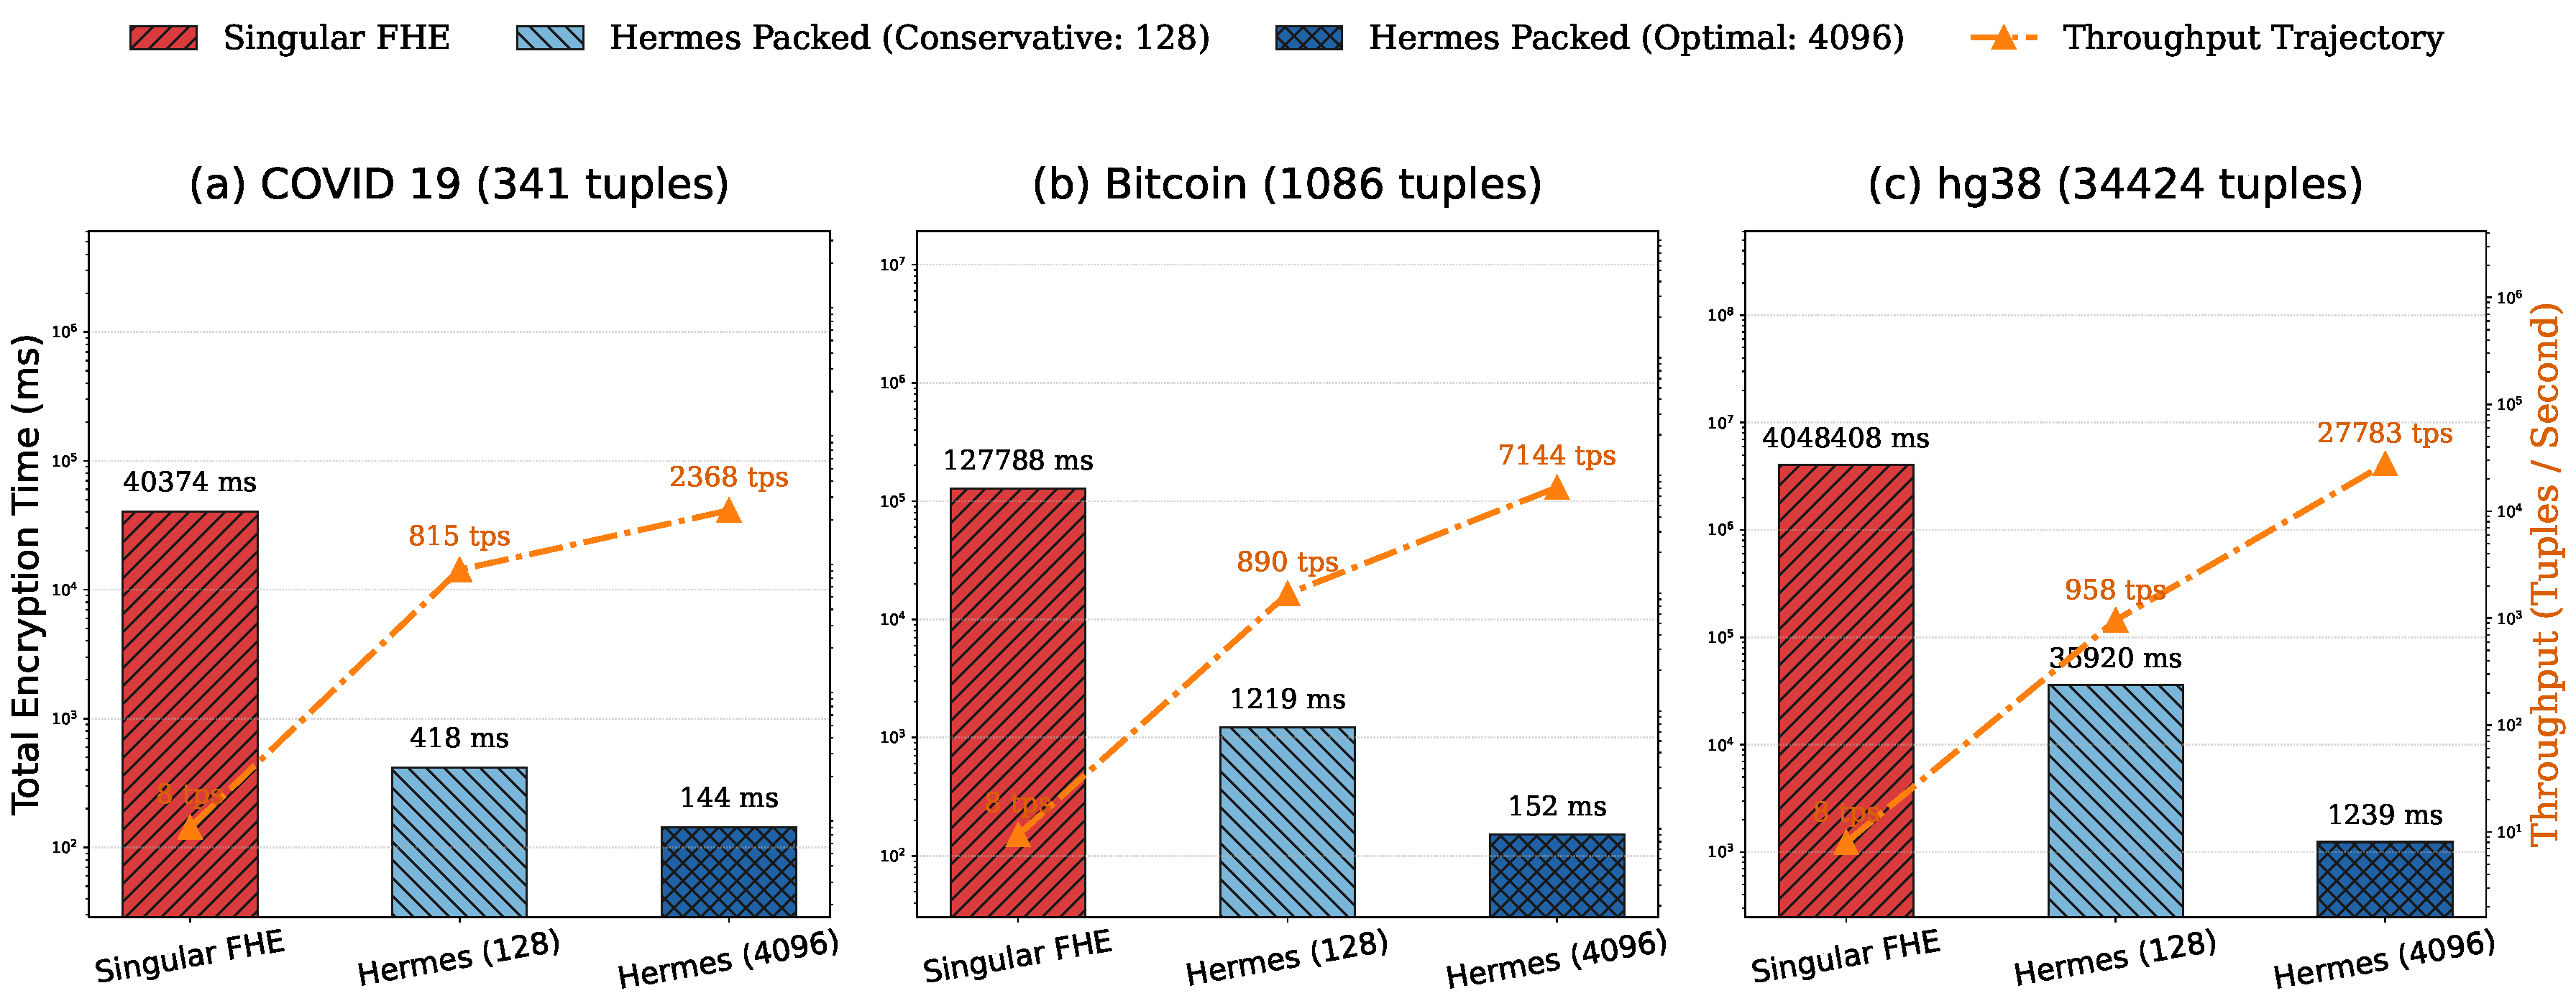
\includegraphics[width=\columnwidth]{fig/eval_encryption.pdf}
\caption{Encryption throughput and absolute time comparison across three datasets. 
% Subfigures (a), (b), and (c) display the evaluation for the Singular FHE baseline, the conservative Hermes configuration at 128 slots, and the optimal Hermes configuration at 4096 slots. The left vertical axes and bars represent absolute encryption time in milliseconds. The right vertical axes and the overlaid line graphs track the processing throughput measured in tuples per second (tps). All vertical axes utilize a logarithmic scale.
}
\label{fig:encryption}
\end{figure}

The Singular FHE baseline forces the database to generate an independent ciphertext for every single tuple. As shown in Figure~\ref{fig:encryption}(c), encrypting the hg38 dataset tuple by tuple consumes over 4048 seconds, yielding a slow throughput of merely 8 tuples per second. By contrast, Hermes leverages the SIMD capabilities of the BFV scheme to pack multiple relational tuples into a single ciphertext. Even under the most conservative structural configuration of 128 slots, the encryption time for hg38 drops to 35 seconds, boosting the throughput to 958 tuples per second.

When operating at the optimal packing scale of 4096 slots, Hermes reduces the total encryption time for hg38 to 1.2 seconds. The overlaid throughput trajectory highlights this dramatic efficiency gain, revealing a high processing rate of 27783 tuples per second. Similar computational boundaries are observed in the Bitcoin and COVID-19 datasets. These measurements confirm that the vectorized data model successfully reduces the fundamental throughput bottleneck of applying homomorphic encryption to relational database systems.

\subsection{In-Place Update Latency}
\label{sec:eval_update}

To answer RQ2, we evaluate the system performance for in-place data modifications. We focus on the amortized latency per tuple to accurately reflect the throughput capabilities of the vectorized packing architecture under bulk operation workloads.

\begin{figure}[!t]
\centering
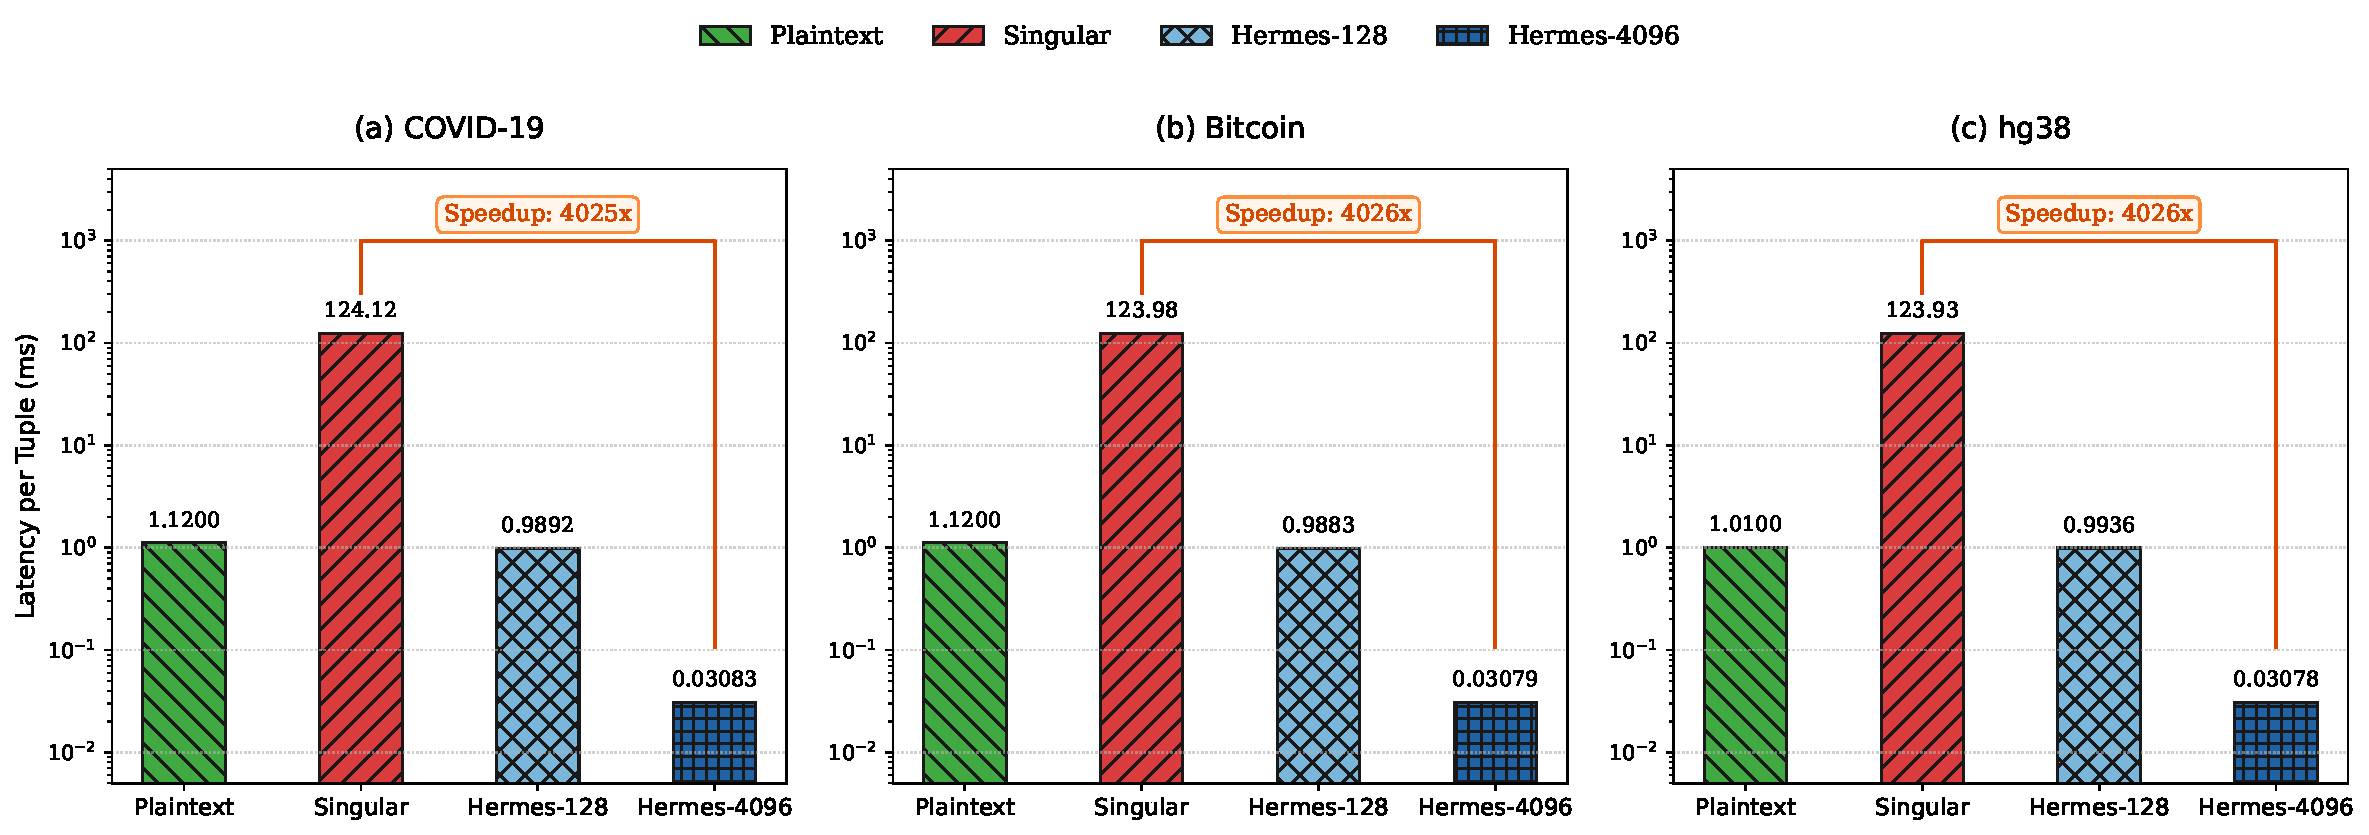
\includegraphics[width=\columnwidth]{fig/eval_insert.pdf}
\caption{Amortized in-place insertion latency per tuple across three evaluation datasets. 
% The vertical axes utilize a logarithmic scale. The floating labels denote the relative speedup of Hermes-4096 against the Singular FHE baseline.
}
\label{fig:insert}
\end{figure}

\begin{figure}[!t]
\centering
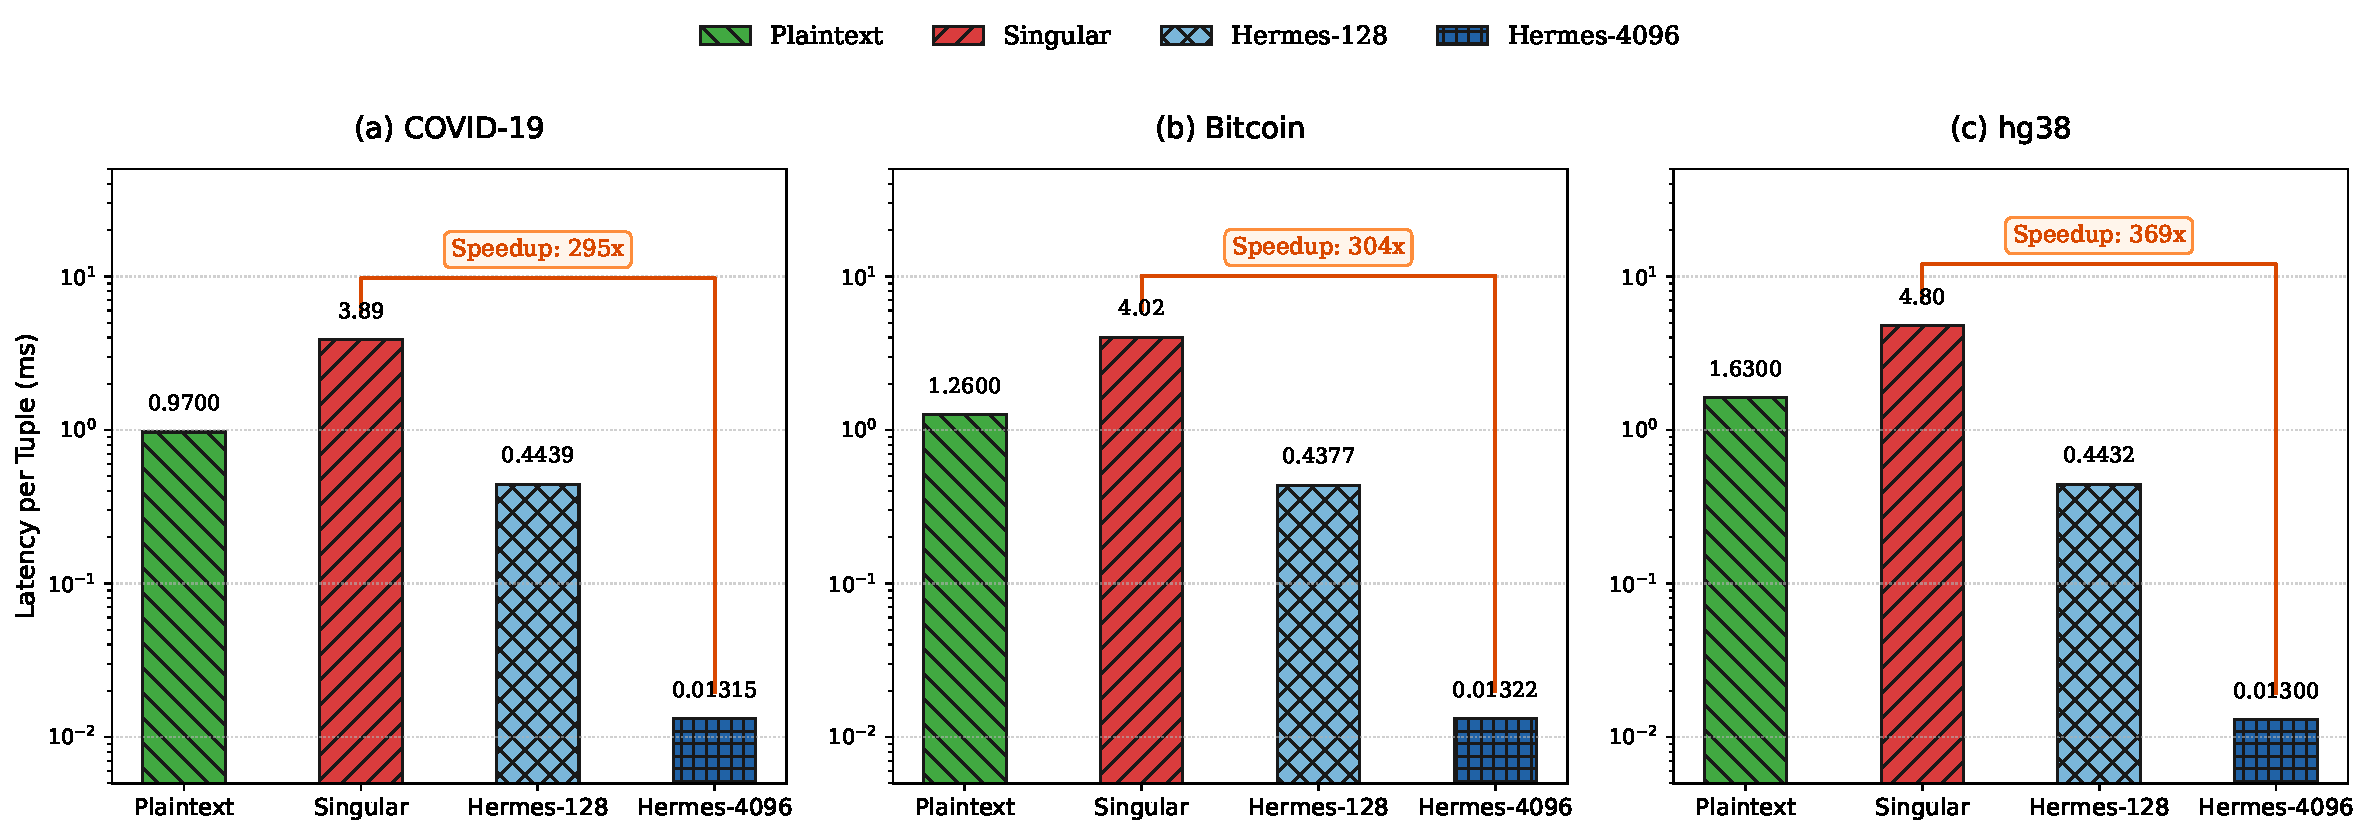
\includegraphics[width=\columnwidth]{fig/eval_remove.pdf}
\caption{Amortized in-place deletion latency per tuple across three evaluation datasets. 
% The vertical axes utilize a logarithmic scale. The floating labels denote the relative speedup of Hermes-4096 against the Singular FHE baseline.\don{The `Speedup' line needs to be elevated: it's cutting the numbers.}
}
\label{fig:remove}
\end{figure}

Figure~\ref{fig:insert} presents the amortized latency for insertion operations. The Singular FHE baseline exhibits a severe bottleneck, requiring approximately 124 milliseconds to insert a single tuple. This delay stems from the mathematical requirement to generate a complete polynomial ciphertext for every isolated record. Hermes leverages the SIMD slots to distribute this cryptographic overhead. Under the optimal configuration of Hermes-4096, the amortized insertion time is reduced to approximately 0.03 milliseconds per tuple. This structural advantage translates to an over 4000x speedup for the Bitcoin dataset and similar gains across the other workloads.

Figure~\ref{fig:remove} illustrates the performance of deletion operations. In the Singular FHE system, a deletion is a direct SQL drop operation requiring merely 4 milliseconds. Hermes cannot physically drop rows within a packed ciphertext and must instead execute homomorphic masking to erase specific slots. Although a single packed deletion takes around 54 milliseconds to compute, amortizing this operation across 4096 slots yields an effective latency of 0.013 milliseconds per tuple. As highlighted by the overlaid metrics, this results in a 369x speedup over the singular approach for the hg38 dataset. Other two datasets show similar trends, leading to speedups around 300x.

These empirical results validate that the SIMD packing design does not degrade the practical update performance. By amortizing the cryptographic polynomial operations across thousands of relational tuples, Hermes successfully maintains sub-millisecond effective latencies for both insertions and deletions.

\subsection{Cryptographic Aggregation Queries}
\label{sec:eval_microbenchmarks}

To answer RQ3, we evaluate the performance of Hermes on aggregation queries. To isolate the intrinsic cryptographic efficiency of our data model from the inherent execution overhead of the MySQL engine, we conduct these evaluations at the core operator level. Although Hermes natively processes SQL aggregations, measuring them end-to-end would introduce parsing and scheduling artifacts that obscure the pure cryptographic throughput. Therefore, we implement this section's benchmarks as standalone C++ programs. This approach allows us to directly compare our rotation-free aggregation technique against traditional cryptographic methods under strict computational isolation.
All benchmarks are executed with $N=2^{14}$ and $t=65537$, yielding 8192 slots.

\begin{figure}[!t]
\centering
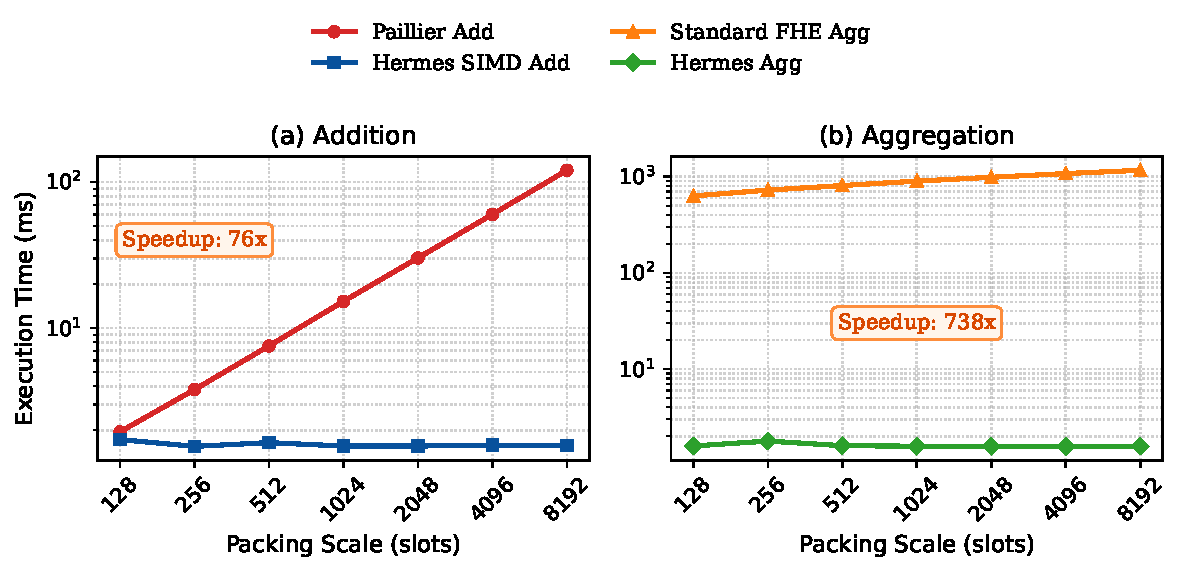
\includegraphics[width=\linewidth]{fig/eval_microbenchmarks.pdf}
\caption{Cryptographic microbenchmarks comparing (a) vector-add throughput against Intel-accelerated Paillier and (b) Hermes rotation-free aggregation against the standard logarithmic-rotation FHE baseline. 
% Both vertical axes use a logarithmic scale.
}
\label{fig:microbenchmarks}
\end{figure}

Figure~\ref{fig:microbenchmarks}(a) compares the throughput of encrypted addition between the proposed Hermes data model and the Intel Paillier Cryptosystem Library (IPCL)~\cite{ipcl_github}. While Paillier is a highly optimized partially homomorphic scheme, its scalar nature requires $n$ separate ciphertext additions to process $n$ tuples. As the packing scale increases to 8192 slots, Paillier's latency grows linearly to 120.5 ms. In contrast, Hermes utilizes the SIMD capabilities of BFV to perform a single vector-add operation that processes all 8192 slots simultaneously. This results in a near-constant latency of 1.57 ms, representing a 76x throughput advantage at the maximum scale.

Figure~\ref{fig:microbenchmarks}(b) evaluates the scalability of encrypted aggregation. Standard FHE aggregation strategies rely on a sequence of $\log n$ Galois rotations and relinearizations to sum internal slots. At 8192 slots, this conventional approach consumes over 1165 ms per ciphertext. Hermes fundamentally bypasses this bottleneck by embedding a precomputed local sum into a reserved auxiliary slot during the packing phase. Global aggregation in Hermes is thus reduced to a single ciphertext-level addition over these auxiliary slots. As shown in the results, Hermes completes the same aggregation in 1.58 ms, achieving a 738x speedup over the rotation-based baseline.

These microbenchmarks demonstrate that the performance gains in Hermes are not merely implementation-level optimizations but stem from a structural shift in how homomorphic primitives are applied to relational data. By aligning the database layout with the algebraic invariants of SIMD-FHE, Hermes transforms traditionally expensive cryptographic tasks into constant-time operations.

\subsection{Scalability of Packing Granularity}
\label{sec:eval_scalability}

\begin{figure}[!t]
\centering
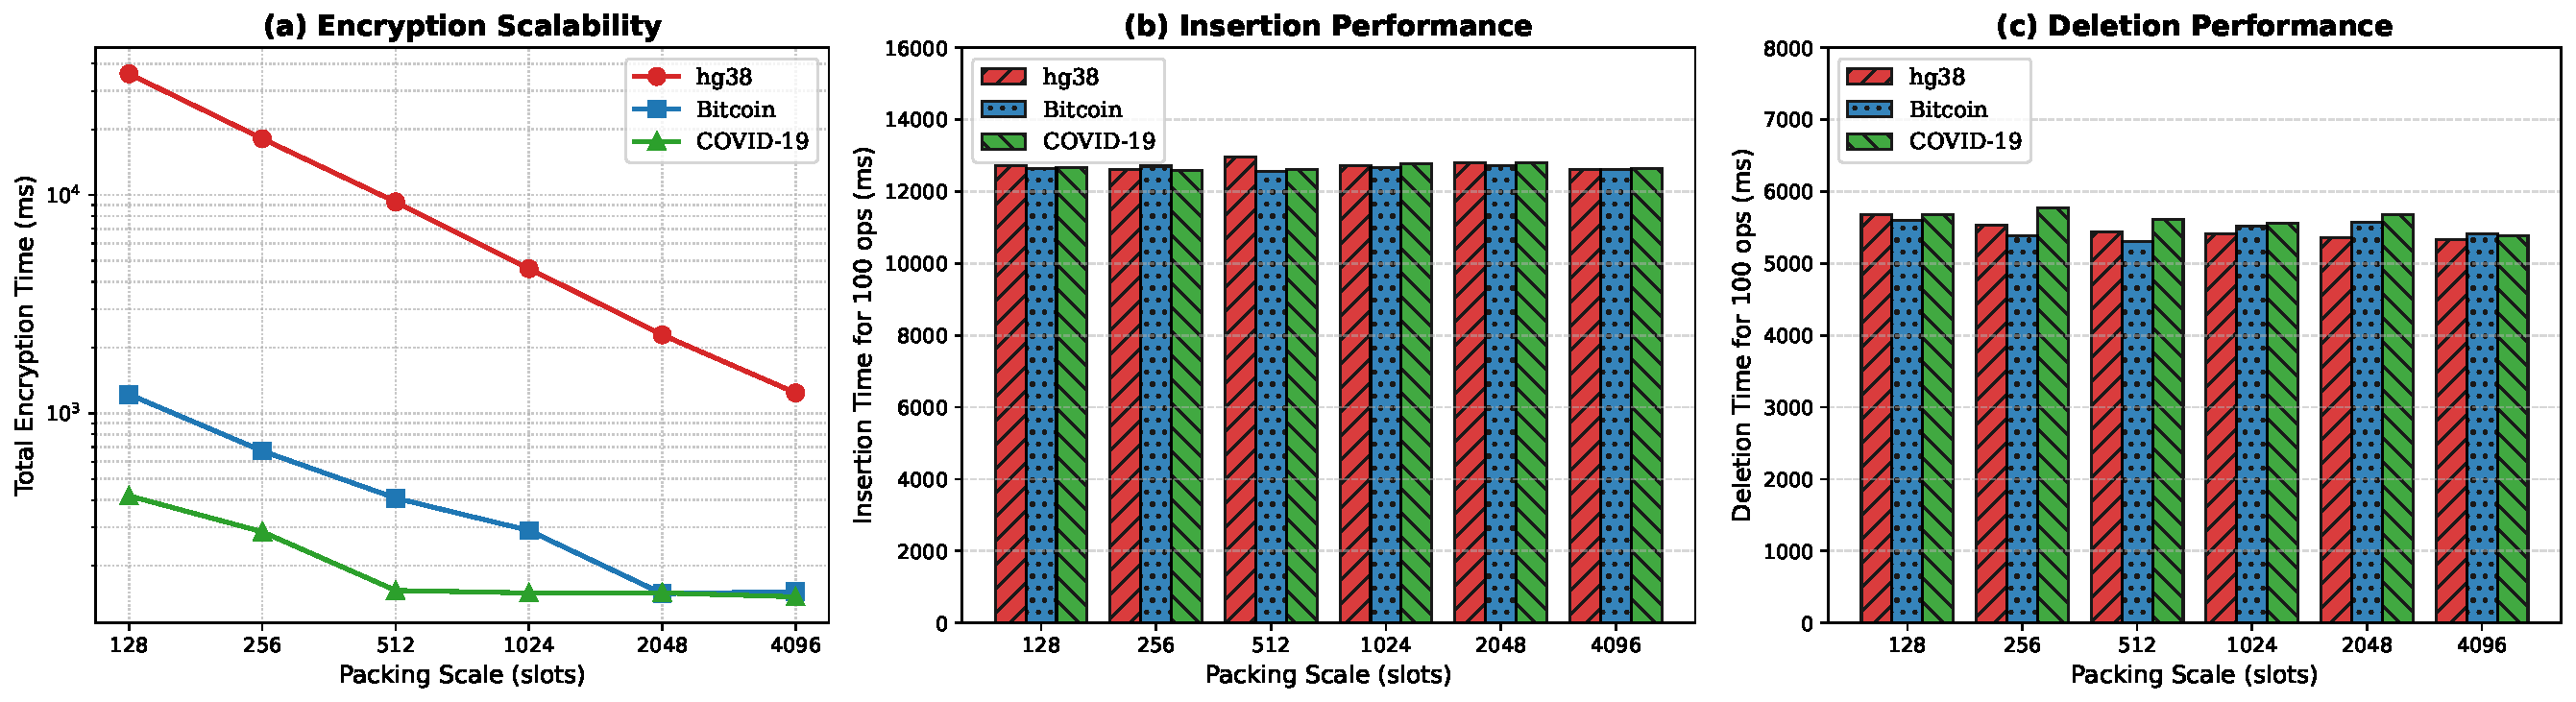
\includegraphics[width=\columnwidth]{fig/eval_scalability.pdf}
\caption{Performance scalability of Hermes across varying packing scales from 128 to 4096 slots. 
% Subfigure (a) shows the total encryption time in a log-log scale. Subfigures (b) and (c) display the execution time for 100 in place insertions and deletions respectively.
}
\label{fig:scalability}
\end{figure}

To address RQ4, we analyze the system performance across different logical group capacities ranging from 128 to 4096 slots. Figure~\ref{fig:scalability} illustrates the execution latency for encryption, insertion, and deletion operations under varying packing scales.

Figure~\ref{fig:scalability}(a) demonstrates a clear inverse relationship between the packing scale and the total encryption time. As the packing capacity doubles, the number of required physical ciphertexts is reduced by half. This leads to an exponential reduction in the overall cryptographic overhead. For example, encrypting the complete hg38 dataset takes over 35 seconds with a pack size of 128 but drops to approximately 1.2 seconds when the scale expands to 4096. This validates the design philosophy that maximizing the utilization of plaintext slots effectively amortizes the initial data ingestion latency.

Conversely, Figure~\ref{fig:scalability}(b) and Figure~\ref{fig:scalability}(c) reveal that the performance of in-place modifications remains entirely decoupled from the packing scale. The time required to perform 100 insertions or 100 deletions stays roughly constant across all scales. Specifically, the batch insertions stabilize at approximately 12.6 seconds, while the corresponding deletions take about 5.4 seconds. 
This constant time complexity is a direct manifestation of the underlying homomorphic mechanics. Because the polynomial ring dimension is fixed at $N=2^{14}$ during the cryptographic context initialization, the computational cost of shifting and masking operations depends solely on the algebraic structure rather than the logical payload. Processing a ciphertext containing 128 active slots requires the exact same CPU cycles as processing one with 4096 active slots. Consequently, system administrators can safely maximize the packing scale to optimize storage footprints and encryption throughput without incurring any latency penalties during subsequent data modifications.

\section{Conclusion and Future Work}
\label{sec:conclusion}

\don{TODO}

% \section*{Acknowledgments}

% Results presented in this paper were obtained using the Chameleon testbed supported by the National Science Foundation.

\bibliographystyle{ACM-Reference-Format}
\bibliography{ref}

\newpage
\appendix

\section{Appendix}

\subsection{Full Proofs}

\begin{lemma}
Let $\mathcal{C}$ be the set of ciphertexts generated and manipulated by Hermes. Then under the assumption that the base FHE scheme (BFV) is IND-CPA secure, the ciphertext $c \in \mathcal{C}$ remains IND-CPA secure throughout all operations in Hermes.
\end{lemma}

\begin{proof}
The proof proceeds by reduction. Suppose there exists an adversary $\mathcal{A}_\text{Hermes}$ that can distinguish two ciphertexts $c_0, c_1 \in \mathcal{C}$ produced under Hermes’ operations with non-negligible advantage. Then we construct an adversary $\mathcal{A}_\text{BFV}$ that breaks IND-CPA security of the underlying BFV scheme.

We consider the following components:
\begin{itemize}
  \item \textbf{Packing}: When packing multiple values into a single ciphertext, we construct a vector $v = (v_0, \dots, v_{n-2}, s)$ where $s = \sum_{i=0}^{n-2} v_i$. The encryption $\mathsf{Enc}(v)$ is indistinguishable from $\mathsf{Enc}(v')$ for any $v'$ of same dimension, as this reduces to IND-CPA security over vector plaintexts in BFV.

  \item \textbf{Auxiliary Slot}: Including a local sum $s$ in the last slot of the plaintext vector does not affect security, since $s$ is deterministically computed from values already encrypted. Its inclusion does not leak new information beyond what is already present in the vector.

  \item \textbf{Insertion}: To insert a plaintext $v$ into a packed ciphertext $c$, we encrypt $v$ into a ciphertext $c_v$, construct a plaintext mask $m$ with $m[i] = 1$, and compute $c' = c + \mathsf{EvalMult}(c_v, m)$. The resulting $c'$ remains IND-CPA secure because it is the sum of IND-CPA secure ciphertexts and homomorphic evaluations thereof. The slot mask $m$ is public and fixed, so no leakage is introduced.

  \item \textbf{Deletion}: Similar reasoning applies. The rotated ciphertext and masked-out tail are both outputs of deterministic homomorphic operations on encrypted data, preserving indistinguishability under the semantic security of BFV.

  \item \textbf{Aggregation}: Aggregation over auxiliary slots only involves ciphertext addition. Since BFV supports additive homomorphism, and all ciphertexts involved are IND-CPA secure, the sum remains indistinguishable.
\end{itemize}

Thus, any distinguishing advantage of $\mathcal{A}_\text{Hermes}$ implies an advantage in distinguishing $\mathsf{Enc}(v)$ vs $\mathsf{Enc}(v')$, contradicting the IND-CPA security of BFV.
\end{proof}

\begin{theorem}
If the underlying BFV encryption scheme is IND-CPA secure, then Hermes satisfies slot-update indistinguishability for any polynomial-time adversary $\mathcal{A}$.
\end{theorem}

\begin{proof}
We reduce the problem to the IND-CPA security of BFV and the semantic uniformity of the masking and shift primitives. Let $m_{i}$ be a plaintext mask such that $m_{i}[j] = \delta$ if $j = i$, and $0$ otherwise. The insertion operation computes:
\[
c' = \mathsf{EvalAdd}(c_{\text{shifted}}, \mathsf{EvalMult}(c_\delta, m_i)),
\]
where $c_{\text{shifted}}$ is the result of a homomorphic rotation and masking on $c$ that preserves all but slot $i$.

Because $c_\delta = \mathsf{Enc}(\delta)$ is fresh and semantically secure under BFV, and $m_i$ is public and independent of $\delta$, the term $\mathsf{EvalMult}(c_\delta, m_i)$ remains indistinguishable regardless of the value of $i$. The subsequent addition with $c_{\text{shifted}}$ is also homomorphic and does not reveal slot index, since the masked slots are zeroed out beforehand. As a result, the output ciphertext $c'$ is statistically indistinguishable whether insertion occurred at $i_0$ or $i_1$.

If $\mathcal{A}$ had non-negligible advantage in distinguishing $i_0$ from $i_1$, we could construct a distinguisher $\mathcal{B}$ that breaks IND-CPA security by embedding $i_b$ into the encryption pattern. This contradicts our assumption.
\end{proof}

\begin{theorem}
  Hermes guarantees the following three properties for any sequence of homomorphic insertions, deletions, and global aggregations over packed ciphertexts:
  \begin{enumerate}
    \item The logical payload vector within each ciphertext remains consistent with the intended insertions and deletions, preserving the correct order and values of active slots.
    \item The auxiliary sum slot accurately reflects the current sum of all valid payload slots after any sequence of updates, ensuring that local statistics remain correct.
    \item The result of encrypted aggregation (e.g., $`SUM'$) over multiple ciphertexts yields the correct aggregate value corresponding to the underlying plaintexts, even in the presence of concurrent updates.
  \end{enumerate}
\end{theorem}

\begin{proof}

We assume a ciphertext $c \leftarrow \mathsf{Encrypt}([v_0, \dots, v_{n-2}, \sigma])$, where $v_i \in \mathbb{Z}_t$ is the plaintext payload at slot $i$ and $\sigma = \sum_{i=0}^{n-2} v_i$ is the precomputed local sum stored in the auxiliary slot $n-1$.

\paragraph{(1) Correctness of Homomorphic Insertion.}
Let $v_{\text{new}} \in \mathbb{Z}_t$ be a value inserted into position $i$ (with $0 \leq i \leq n-2$). Define the updated plaintext vector as:
\[
[v_0', \dots, v_{n-2}'] = [v_0, \dots, v_{i-1}, v_{\text{new}}, v_i, \dots, v_{n-3}]
\]
The homomorphic insertion process rotates the suffix 
\[\{v_i, \dots, v_{n-2}\}\] 
one position to the right using a Galois automorphism, masks the insertion point $i$ with a one-hot vector $m^{(i)} \in \mathbb{Z}_t^n$ such that $m^{(i)}[i] = 1$ and $0$ elsewhere, and adds $v_{\text{new}} \cdot m^{(i)}$ via plaintext multiplication.
Let $c_{\text{ins}} = \mathsf{EvalAdd}(c_{\text{shifted}}, \mathsf{EvalMult}(\mathsf{Encrypt}(v_{\text{new}}), m^{(i)}))$. 
Then, under correct decryption:
\[
\mathsf{Decrypt}(c_{\text{ins}})[j] =
\begin{cases}
v_j & \text{if } j < i \\
v_{\text{new}} & \text{if } j = i \\
v_{j-1} & \text{if } i < j \leq n-2 \\
\sigma + v_{\text{new}} & \text{if } j = n-1
\end{cases},
\]
which matches the intended semantics. 
Note that the local sum is homomorphically updated by
\[
\sigma' = \sigma + v_{\text{new}} \in \mathbb{Z}_t,
\]
through scalar plaintext addition on the last slot.

\paragraph{(2) Correctness of Homomorphic Deletion.}
Let $v_i$ be deleted from position $i$. The deletion logic performs a Galois rotation that left-shifts all slots $j > i$, then applies a mask $z \in \mathbb{Z}_t^n$ such that $z[n{-}1] = 0$ and $z[j] = 1$ for $j < n-1$, to zero out the stale tail. The resulting ciphertext $c_{\text{del}}$ decrypts to:
\[
\mathsf{Decrypt}(c_{\text{del}})[j] =
\begin{cases}
v_j & \text{if } j < i \\
v_{j+1} & \text{if } i \leq j \leq n-3 \\
0 & \text{if } j = n-2 \\
\sigma - v_i & \text{if } j = n-1
\end{cases},
\]
where $\sigma$ is again updated via scalar subtraction. The vector semantics remain preserved, and auxiliary statistics remain valid.

\paragraph{(3) Correctness of Global Aggregation.}
Let $c^{(1)}, \dots, c^{(k)}$ be a collection of packed ciphertexts, each of form:

\[
\begin{aligned}
c^{(\ell)} &= \mathsf{Encrypt}\left(
  \left[
    v^{(\ell)}_0,\, v^{(\ell)}_1,\, \dots,\, v^{(\ell)}_{n-2},\, \sigma^{(\ell)}
  \right]
\right), \\
\sigma^{(\ell)} &= \sum_{j=0}^{n-2} v^{(\ell)}_j.
\end{aligned}
\]
Then, the encrypted global sum is computed by:
\[
c_{\text{agg}} = \mathsf{EvalAdd}(c^{(1)}, \dots, c^{(k)}),
\]
followed by slot extraction $\mathsf{Extract}(c_{\text{agg}}, n-1)$ to isolate the final aggregated value. 

The decrypted result satisfies:
\[
\mathsf{Decrypt}(c_{\text{agg}})[n-1] = \sum_{\ell = 1}^{k} \sigma^{(\ell)} = \sum_{\ell = 1}^{k} \sum_{j=0}^{n-2} v_j^{(\ell)},
\]
which matches the true plaintext sum across all tuples.
\end{proof}

\end{document}
